\documentclass[9pt,journal]{IEEEtran}
\usepackage{tikz}
\usepackage[T1]{fontenc}
\usepackage[utf8]{inputenc}
\usepackage{graphicx}
\graphicspath{{./images/}}
\usepackage{mathtools}
\usepackage{amsmath,amsthm,amsfonts,amssymb}
\usepackage{pgfplots}
\usepackage{tabularx}
\usepackage{chngcntr}
\usepackage{float}
\pgfplotsset{width=9cm,compat=1.18}
\counterwithin{figure}{section}
\newcommand\numberthis{\addtocounter{equation}{1}\tag{\theequation}}
\usepackage[linesnumbered,ruled,boxed,commentsnumbered]{algorithm2e}
\newtheorem{lemma}{Lemma}[section]
\newtheorem{theorem}{Teorema}[section]
\newtheorem{definition}{Definición}[section]
\numberwithin{equation}{section}
\renewcommand{\arraystretch}{1.5}
\setcounter{tocdepth}{1}
\usepackage{titlesec}

\setcounter{secnumdepth}{4}

\titleformat{\paragraph}
{\normalfont\normalsize\bfseries}{\theparagraph}{1em}{}
\titlespacing*{\paragraph}
{0pt}{3.25ex plus 1ex minus .2ex}{1.5ex plus .2ex}

\title{Raíces de funciones irracionales.}

\author{
    Ernesto José Canales Guillén (00051120@uca.edu.sv)\\
    Víctor Daniel Peraza Bolaños (00143320@uca.edu.sv)\\
    Diego Fernando Ramos Guardado (00043920@uca.edu.sv)\\
    Laura Ivonne Shahidinejad Martínez (00365919@uca.edu.sv)
}

\begin{document}

\maketitle
\tableofcontents
\section{Método de la secante.}
\subsection{Deducción y descripción del método}
\subsubsection{Deducción}
En el método de Newton Raphson, se necesita saber la derivada de la función en cada aproximación. La fórmula para hallar el siguiente punto en dicho método es la siguiente:

\begin{equation}
p_n = p_{n-1} - \frac{f(p_{n-1})}{f'(p_{n-1})}
\end{equation} 

Conocer la derivada de la función puede resultar más complejo, por lo que, en lugar de la derivada, se puede utilizar la siguiente aproximación:

\begin{gather*}
f'(p_{n-1}) = \lim_{x\to p_{n-1}} \frac{f(x) - f(p_{n-1})}{x-p_{n-1}} 
\end{gather*}

Si $P_{n-2}$ está cerca de $P_{n-1}$, entonces tenemos lo siguiente:

\begin{gather*}
f'(p_{n-1}) \approx \frac{f(p_{n-2})-f(p_{n-1})}{p_{n-2}-p_{n-1}} = \frac{f(p_{n-1})-f(p_{n-2})}{p_{n-1}-p_{n-2}}
\end{gather*}

Al sustituir la aproximación de $f'(P_{n-1})$ en la fórmula (1), tenemos la fórmula del método de la secante \cite{Burden_English}:

\begin{gather*}
p_n = p_{n-1} - \frac{f(p_{n-1})}{\frac{f(p_{n-1})-f(p_{n-2})}{p_{n-1}-p_{n-2}}}
\end{gather*}

\begin{equation}
p_n = p_{n-1} - \frac{f(p_{n-1})(p_{n-1}-p_{n-2})}{f(p_{n-1})-f(p_{n-2})} 
\end{equation}


A diferencia de Newton, en el método de la secante se necesitan dos puntos iniciales $P_{n-2}$ y $P_{n-1}$. Al utilizar la fórmula de la secante, se encuentra el siguiente punto Pn. 

Después se modifica la notación para encontrar $P_{n+1}$ utilizando los dos puntos anteriores $P_{n-1}$ y $P_n$, y así sucesivamente hasta encontrar la raíz.

\subsubsection{Descripción}
El método de la secante sirve para encontrar raíces de ecuaciones sin saber la derivada de la función (a diferencia del método de Newton en dónde sí es necesario conocer la derivada). La raíz de una ecuación no es otra cosa más que el valor de la $X$ cuando $f(x)$ vale cero. Es decir que este método es una modificación del método de Newton.

¿Cómo funciona?

El método de la secante requiere dos puntos iniciales $P_{n-2}$ (valor más pequeño) y $P_{n-1}$ (valor más grande). Esos dos valores sirven para generar una línea recta que va a cruzar con el eje de las $X$ y justamente ese punto se va a conocer como $P_n$ o la aproximación a la raíz.

Después de utilizar la fórmula para encontrar $P_n$, se modifica la notación para encontrar $P_{n+1}$ utilizando los dos puntos anteriores $P_{n-1}$ y $P_n$, y así sucesivamente hasta encontrar la raíz o al menos hasta que el error sea menor o igual a la tolerancia. 

No se necesita otra cosa más que la función y proponer los dos valores de inicio para tener la aproximación. A diferencia del método de newton, no se ocupa la derivada.


\subsection{Análisis del error y demostración de convergencia}

Se asume que $r$ es una raíz para $f(x)=0$. La secuencia ${x_n}$ del método de la secante está dada por: 

\begin{gather*}
x_{n+1 }= x_{n} - \frac{f(x_{n})(x_{n}-x_{n-1})}{f(x_{n})-f(x_{n-1})} 
\end{gather*}

Se quiere encontrar el exponente $p$ de tal manera que:

\begin{gather*}
\lim_{n\to \infty} \frac{|x_{n+1}-r|}{|x_n - r|^{p}} = \lim_{n\to \infty} \frac{|e_{n+1}|}{|e_n|^{p}} = \lambda
\end{gather*}

En donde $e_n = x_n - r$. Por el teorema de Taylor,

\begin{gather*}
f(x_{n-1})= f(e_{n-1}+r) = f(r)+e_{n-1}f'(r) \\
+\frac{e^{2}_{n-1}}{2}f''(r)+O(e^{3}_{n-1})
\end{gather*}

\begin{gather*}
f(x_{n})= f(e_n+r) = f(r)+e_{n}f'(r)+\frac{e^{2}_n}{2}f''(r)+O(e^{3}_n)
\end{gather*}

Ya que $f(r)=0$, se tiene para $e=e_n$ o $e=e_{n-1}$

\begin{gather*}
f(e+r)= e f'(r)+\frac{e^{2}}{2}f''(r)+O(e^{3})
\end{gather*}

\begin{gather*}
f(e+r) \approx e f'(r)+\frac{e^{2}}{2}f''(r)
\end{gather*}

El método de la secante da:

\begin{gather*}
x_{n+1 }= x_{n} - \frac{f(x_{n})(x_{n}-x_{n-1})}{f(x_{n})-f(x_{n-1})} 
\end{gather*}

\begin{gather*}
\Rightarrow e_{n+1}+r= e_{n} + r - f(e_n + r) \frac{(e_n +r) -(e_{n-1}+r)}{f(e_n + r)-f(e_{n-1} + r)} 
\end{gather*}

\begin{equation}
\Rightarrow e_{n+1}= e_{n} - \frac{f(e_n + r)(e_n - e_{n-1})}{f(e_n + r)-f(e_{n-1} + r)} 
\end{equation}\\

Dejando:\\

\begin{gather*}
M= \frac{f''(r)}{2f'(r)} \Leftrightarrow \frac{f''(r)}{2} = Mf'(r)
\end{gather*}\\\\

Ignorando los términos de orden superior, el numerador de la ecuación (3) se convierte en lo siguiente:

\begin{gather*}
    f(e_n +r)(e_n - e_{n-1})= (e_nf'(r)+\frac{e^{2}_n}{2}f''(r))(e_n -e_{n-1}) \\
    = (e_nf'(r)+Me^{2}_nf'(r))(e_n -e_{n-1}) \\
    = e_nf'(r)(1+Me_n)(e_n -e_{n-1})
\end{gather*} 

El denominador de la ecuación (3) se convierte en:


\begin{gather*}
    f(e_n +r)-f(e_{n-} +r)= [e_nf'(r)+\frac{1}{2}f''(r)e^{2}_n][e_{n-1}f'(r) \\
    +\frac{1}{2}f''(r)e^{2}_{n-1}] \\
    = f'(r)(e_n-e_{n-1})+\frac{1}{2}f''(r)(e^{2}_n -e^{2}_{n-1}) \\
    = f'(r)(e_n-e_{n-1})+Mf'(r)(e^{2}_n -e^{2}_{n-1}) \\
    = f'(r)(e_n-e_{n-1})(1+M(e_n +e_{n-1})) \\
\end{gather*}


Por lo tanto, la ecuación (3) ahora es:


\begin{gather*}
    e_{n+1}= e_{n} - \frac{e_nf'(r)(1+Me_n)(e_n -e_{n-1})}{f'(r)(e_n-e_{n-1})(1+M(e_n +e_{n-1}))} \\
    = e_{n} - \frac{e_n(1+Me_n)}{1+M(e_n+e_{n-1})} \\
    = \frac{e_n+e_n M(e_n+e_{n-1})-e_n(1+Me_n)}{1+M(e_n+e_{n-1})} \\
    = \frac{M e_n e_{n-1}}{1+M(e_n+e_{n-1})} \\
\end{gather*}


Lo cual implica que:

\begin{gather*}
    e_{n+1} \approx M e_n e_{n-1} \approx \frac{f''(r)}{2f'(r)} e_n e_{n-1}
\end{gather*}

Ahora se calcula el exponente $p$. Se tiene $|e_{n+1}= \lambda|e_n|^{p}$ y $|e_{n+1} \approx |M||e_n||e_{n-1}|$, entonces:

\begin{gather*}
    \lambda|e_n|^{p}=|M||e_n||e_{n-1}| \\
    \Rightarrow |e_n|^{p-1}=|M/\lambda||e_{n-1}| \\
    \Rightarrow |e_n|=|M/\lambda|^{1/{p-1}}|e_{n-1}|^{1/{p-1}}= \lambda|e_{n-1}|^{p} \\
\end{gather*} 

Por lo que se obtiene \cite{edwards}:

\begin{gather*}
    p=\frac{1}{p-1} \Rightarrow p^{2}-p-1=0 \Rightarrow p = \frac{1+ \sqrt{5}}{2}
\end{gather*} 

La convergencia de este método es superlineal, lo que significa que es mayor que los de convergencia linear pero menor que los de convergencia cuadrática como el método de Newton.

En este caso, $p$ es el número de oro, aproximadamente $1.618$, lo que significa que el método de la secante es casi tan rápido como Newton-Raphson pero un poco más lento y que es más rápido que los de convergencia lineal.

\subsection{Análisis sobre la eficiencia del método}

El método de la secante es iterativo, requiere la función y los dos puntos anteriores para encontrar $Pn$ o la raíz, utiliza la recta secante que pasa por los puntos que le corresponden a las aproximaciones anteriores y puede resultar más fácil de utilizar a comparación del método de Newton, sin embargo el método de la secante no siempre converge, es decir que no necesariamente se encontrará una aproximación de la solución que se está buscando.  Además, no necesariamente se tiene una referencia al elegir los dos puntos iniciales y si estos no son ideales, el método no resultará muy eficiente. 

Como se mencionó anteriormente, el método puede diverger como por ejemplo, si se tienen dos puntos iniciales ($X_0$ y $X_1$), se calculan sus imágenes y la recta que los contiene, y como resultado se obtiene una recta paralela al eje $x$, es decir, una recta que nunca va a interceptar al eje $x$, en este caso el método diverge. Algebraicamente, se estaría obteniendo una división entre cero. También se pueden tener variaciones de eso, no obteniendo una recta paralela exactamente al eje $x$, pero que se va a interceptar en el infinito, en un número muy grande o muy pequeño.


Otro caso de divergencia es cuando en lugar de irse acercando a la solución que se busca, más bien se está alejando. Gráficamente es muy sencillo ver cuándo el método va a diverger, porque no nos estamos acercando al cero, es decir, a la intercepción de la función con el eje $x$. Algebraicamente, se debe ver si el error está aumentando o disminuyendo. Si el error disminuye, el método está convergiendo y si está aumentando entonces el método probablemente esté divergiendo. 


\subsection{Ventajas y desventajas}

\subsubsection{Ventajas}

\begin{itemize}
  \item En el método de Newton, se ocupa la derivada de la función lo cual resulta en más operaciones aritméticas y se vuelve más complejo. A diferencia del método de Newton, en el método de la secante no se ocupa la derivada de la función.
  \item Solo se necesita conocer la función y proponer dos puntos iniciales, se sustituyen en la función y lo mismo se repite hasta encontrar la raíz.
  \item Es menos complejo que otros métodos que requieren más pasos y operaciones para obtener resultados.
\end{itemize}

\subsubsection{Desventajas}

\begin{itemize}
  \item La convergencia del método de la secante es ligeramente más lenta que la del método de Newton. 
  \item Un problema que se tiene con la aplicación del método de la secante es la posibilidad de que el polinomio tenga raíces complejas incluso cuando todos los coeficientes son números reales. 
  \item La agrupación de raíces no está garantizada para el método de la secante.
  \item Se necesitan dos valores iniciales, entonces tenemos más probabilidad de que este método numérico no sea convergente. Al contrario, Newton al solo tener un valor inicial Xo tiene más probabilidad de converger.
  \item No siempre converge, es decir que no necesariamente se va a encontrar una aproximación de la solución que estamos buscando.
  \item El método depende mucho de las condiciones iniciales que se escojan.
\end{itemize}

\subsection{Pseudocódigo}

\begin{algorithm}
    \SetKwComment{Comment}{/}{/}
    
    \caption{Método de la secante} 
    \KwIn{Aproximaciones iniciales $p_0$, $p_1$ tolerancia TOL; número máximo de iteraciones $N_0$.}\
    \KwOut{Solución aproximada \textit{p} o mensaje de error.}
    $i = 2$; 
    \BlankLine
    $q_0 = f(p_0)$; 
    \BlankLine
    $q_1 = f(p_1)$.
    \BlankLine
    \While{$i \le n_0 $}{
        $p = p_1 - q_1(p_1 - p_0)/(q_1-q_0)$
        \If{$|p-p_1| < TOL$}{\tcp{El procedimiento fue exitoso} \Return{p}}
        $i = i + 1$.
        $p_0=p_1$; 
        $q_0=q_1$;
        $p_1=p$;
        $q_1=f(p)$
    }
    \Return \KwOut{"El metodo fallo luego de N iteraciones, N="$N_0$}
    \end{algorithm}

\subsection{Elementos ilustrativos}

Ejemplo gráfico del método de la secante con la función $f(x)=x^2-1$:\\

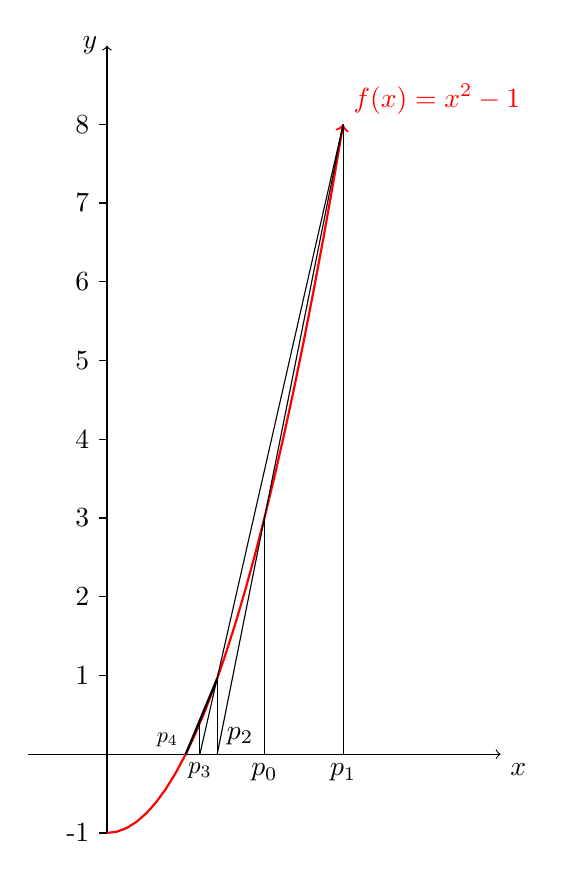
\begin{tikzpicture}[domain=0:2]
    \draw[->] (-1,0) -- (5,0)
    node[below right] {$x$};
    \draw[->] (0,-1) -- (0,9)
    node[left] {$y$};
    \foreach \y in {-1,1,2,3,4,5,6,7,8}
    \draw (0,\y) -- (-0.1,\y) node[left] {\y};
    
    \draw[red,thick,->] plot[domain=0:3] (\x,\x^2-1) 
    node[above right] {$f(x) = x^2-1$};
    
     \coordinate (A) at (2,0);
     \node[below] at (2,0) {$p_0$};
     \coordinate (B) at (3,0);
     \node[below] at (3,0) {$p_1$};
     \coordinate (C) at (1.4,0);
     \node[above right] at (1.4,0) {$p_2$};
     \coordinate (D) at (1.18,0);
     \node[below, scale=0.9] at (1.18,0) {$p_3$};
     \coordinate (E) at (1.00,0);
     \node[above left, scale=0.8] at (1.00,0) {$p_4$};
     \coordinate (F) at (2,3);
     \coordinate (G) at (3,8);
     \coordinate (H) at (1.4,0.96);
     \coordinate (I) at (1.18,0.3924);
     
    \draw (A) -- (F);
    \draw (B) -- (G);
    \draw (G) -- (C);
    \draw (C) -- (H);
    \draw (G) -- (D);
    \draw (D) -- (I);
    \draw[thick] (H) -- (E);
    
\end{tikzpicture}


\subsection{Ejemplos}

\subsubsection{Ejemplo 1}

Utilice el método de la secante para encontrar una solución para $f(x) = e^{-x} - x$, utilizando como puntos iniciales $p_{n-2} = 2$ y $p_{n-1} = 5$. \\
\\\\
\begin{tabularx}{0.4\textwidth} { 
  | >{\arraybackslash}X 
  | >{\arraybackslash}X
  | >{\arraybackslash}X
  | >{\arraybackslash}X
  | >{\arraybackslash}X | }
 \hline
 i & $p_{n-1}$ & $p_{n-2}$ & $f(p_{n-1})$ & $f(p_{n-2})$ \\
 \hline
 1 & 5 & 2 & -4.99 & -1.86 \\
 \hline
 2 & 0.21 & 5 & 0.60 & -4.99 \\
 \hline
 3 & 0.72 & 0.21 & -0.24 & 0.60 \\
 \hline
 4 & 0.58 & 0.72 & -0.02 & -0.24 \\
 \hline
 5 & 0.57 & 0.58 & 0.00 & -0.02 \\
 \hline
\end{tabularx} \\\\

\begin{tabularx}{0.3\textwidth}{ 
  | >{\arraybackslash}X 
  | >{\arraybackslash}X
  | >{\arraybackslash}X | }
 \hline
 i & $p_{n}$ & ErAbs \% \\
 \hline
 1 & 0.21 & 2258.71  \\
 \hline
 2 & 0.72 & 70.69  \\
 \hline
 3 & 0.58 & 25.25  \\
 \hline
 4 & 0.57 & 1.88  \\
 \hline
 5 & 0.57 & 0.00  \\
 \hline
\end{tabularx} \\\\

Fórmula del método de la secante:

\begin{gather*}
p_n = p_{n-1} - \frac{f(p_{n-1})(p_{n-1}-p_{n-2})}{f(p_{n-1})-f(p_{n-2})} 
\end{gather*} \\

En el caso del error, se puede calcular el error absoluto con la siguiente fórmula:

\begin{gather*}
    EA = |\frac{p_n - p_{n-1}}{p_n}|*100
\end{gather*} \\

\paragraph{Iteración 1}
\begin{gather*}
    f(x) = e^{-x} - x \\
    f(p_{n-1}) = e^{-5} - 5 = -4.99 \\
    f(p_{n-2}) = e^{-2} - 2 = -1.86 \\
    p_n = (5)- \frac{(-4.99*(5-2))}{(-4.99-(-1.86))} = 0.21 \\
    Error absoluto = \frac{0.21-5}{0.21}100 = 2258.71
\end{gather*} \\

\paragraph{Iteración 2}
\begin{gather*}
    f(p_{n-1}) = e^{-0.21} - 0.21 = 0.60 \\
    f(p_{n-2}) = e^{-5} - 5 = -4.99 \\
    p_n = (0.21)- \frac{(0.60*(0.21-5))}{(0.60-(-4.99))} = 0.72 \\
    Error absoluto = \frac{0.72-0.21}{0.72}100 = 70.69
\end{gather*} \\

\paragraph{Iteración 3}
\begin{gather*}
    f(p_{n-1}) = e^{-0.72} - 0.72 = -0.24 \\
    f(p_{n-2}) = e^{-0.21} - 0.21 = 0.60 \\
    p_n = (0.72)- \frac{(-0.24*(0.72-0.21))}{(-0.24-(0.60))} = 0.58 \\
    Error absoluto = \frac{0.58-0.72}{0.58}100 = 25.25
\end{gather*} \\

\paragraph{Iteración 4}
\begin{gather*}
    f(p_{n-1}) = e^{-0.58} - 0.58 = -0.02 \\
    f(p_{n-2}) = e^{-0.72} - 0.72 = -0.24 \\
    p_n = (0.58)- \frac{(-0.02*(0.58-0.72))}{(-0.02-(-0.24))} = 0.57 \\
    Error absoluto = \frac{0.57-0.58}{0.57}100 = 1.88
\end{gather*} \\

\paragraph{Iteración 5}
\begin{gather*}
    f(p_{n-1}) = e^{-0.57} - 0.57 = 0.00 \\
    f(p_{n-2}) = e^{-0.58} - 0.58 = -0.02 \\
    p_n = (0.57)- \frac{(0.00*(0.57-0.58))}{(0.00-(-0.02))} = 0.57 \\
    Error absoluto = \frac{0.57-0.57}{0.57}100 = 0.00
\end{gather*} \\

En este ejemplo se puede observar que al utilizar el último $p_n = 0.57$ en la función original, se obtiene $0$, por lo que ya se ha encontrado la raíz. Cabe mencionar que los resultados se han redondeado a dos decimales.


\subsubsection{Ejemplo 2} 
Utilice el método de la secante para encontrar una solución para $f(x) = x^{2} - 3x - 4$, utilizando como puntos iniciales $p_{n-2} = 5$ y $p_{n-1} = 7$. \\\\

\begin{tabularx}{0.4\textwidth} { 
  | >{\arraybackslash}X 
  | >{\arraybackslash}X
  | >{\arraybackslash}X
  | >{\arraybackslash}X
  | >{\arraybackslash}X | }
 \hline
 i & $p_{n-1}$ & $p_{n-2}$ & $f(p_{n-1})$ & $f(p_{n-2})$ \\
 \hline
 1 & 7 & 5 & 24.00 & 6.00 \\
 \hline
 2 & 4.33 & 7 & 1.78 & 24.00 \\
 \hline
 3 & 4.12 & 4.33 & 0.61 & 1.78 \\
 \hline
 4 & 4.01 & 4.12 & 0.04 & 0.61 \\
 \hline
 5 & 4.00 & 4.01 & 0.00 & 0.04 \\
 \hline
\end{tabularx} \\\\

\begin{tabularx}{0.3\textwidth} { 
  | >{\arraybackslash}X 
  | >{\arraybackslash}X
  | >{\arraybackslash}X | }
 \hline
 i & $p_{n}$ & ErAbs \% \\
 \hline
 1 & 4.33 & 61.54  \\
 \hline
 2 & 4.12 & 5.18  \\
 \hline
 3 & 4.01 & 2.81  \\
 \hline
 4 & 4.00 & 0.18  \\
 \hline
 5 & 4.00 & 0.00  \\
 \hline
\end{tabularx} \\\\


\paragraph{Iteración 1}
\begin{gather*}
    f(x) =x^{2}-3x-4 \\
    f(p_{n-1}) =(7)^{2}-3(7)-4 = 24 \\
    f(p_{n-2}) =(5)^{2}-3(5)-4 = 6 \\
    p_n = (7)- \frac{(24*(7-5))}{(24-6)} = 4.33 \\
    Error absoluto = \frac{4.33-7}{4.33}100 = 61.54 
\end{gather*} \\

\paragraph{Iteración 2}
\begin{gather*}
    f(p_{n-1}) =(4.33)^{2}-3(4.33)-4 = 1.78 \\
    f(p_{n-2}) =(7)^{2}-3(7)-4 = 24 \\
    p_n = (4.33)- \frac{(1.78*(4.33-7))}{(1.78-24)} = 4.12 \\
    Error absoluto = \frac{4.12-4.33}{4.12}100 = 5.18
\end{gather*} \\

\paragraph{Iteración 3}
\begin{gather*}
    f(p_{n-1}) =(4.12)^{2}-3(4.12)-4 = 0.61 \\
    f(p_{n-2}) =(4.33)^{2}-3(4.33)-4 = 1.78 \\
    p_n = (4.12)- \frac{(0.61*(4.12-4.33))}{(0.61-1.78)} = 4.01 \\
    Error absoluto = \frac{4.01-4.12}{4.01}100 = 2.81
\end{gather*} \\

\paragraph{Iteración 4}
\begin{gather*}
    f(p_{n-1}) =(4.01)^{2}-3(4.01)-4 = 0.04 \\
    f(p_{n-2}) =(4.12)^{2}-3(4.12)-4 = 0.61 \\
    p_n = (4.01)- \frac{(0.04*(4.01-4.12))}{(0.04-0.61)} = 4.00 \\
    Error absoluto = \frac{4.00-4.01}{4.00}100 = 0.18
\end{gather*} \\

\paragraph{Iteración 5}
\begin{gather*}
    f(p_{n-1}) =(4.00)^{2}-3(4.00)-4 = 0.00 \\
    f(p_{n-2}) =(4.01)^{2}-3(4.01)-4 = 0.04 \\
    p_n = (4.00)- \frac{(0.00*(4.00-4.01))}{(0.00-0.04)} = 4.00 \\
    Error absoluto = \frac{4.00-4.00}{4.00}100 = 0.00
\end{gather*} \\

En este ejemplo se puede observar que al utilizar el último $p_n = 4.00$ en la función original, se obtiene $0$, por lo que ya se ha encontrado la raíz.

\section{Método de la falsa posición.}
\section{El método de posición falsa (Regula Falsi)}

El método de la falsa posición pretende conjugar la seguridad del método de la bisección con la rapidez del método de la secante.\newline\newline
Como es denominado \cite{Burden_English}, el término Regula Falsi literalmente “regla falsa” o “posición falsa” (a veces es denominado como el método de adivinar y comprobar. \cite{CS_Web}) se refiera a una técnica en la que se usan resultados que se sabe son falsos, pero de algún modo específico, genera aproximaciones de la misma manera que el método de la secante, pero incluye una prueba para garantizar que la raíz siempre se agrupa entre iteraciones sucesivas, para obtener convergencia a un resultado verdadero. Aunque su convergencia está garantizada, tiene una tasa de convergencia lenta.\newline\newline
Los problemas de posición falsa se pueden encontrar en el papiro Rhind, que data de aproximadamente 1650 a.C.

\begin{figure}[!ht]
    \centering
    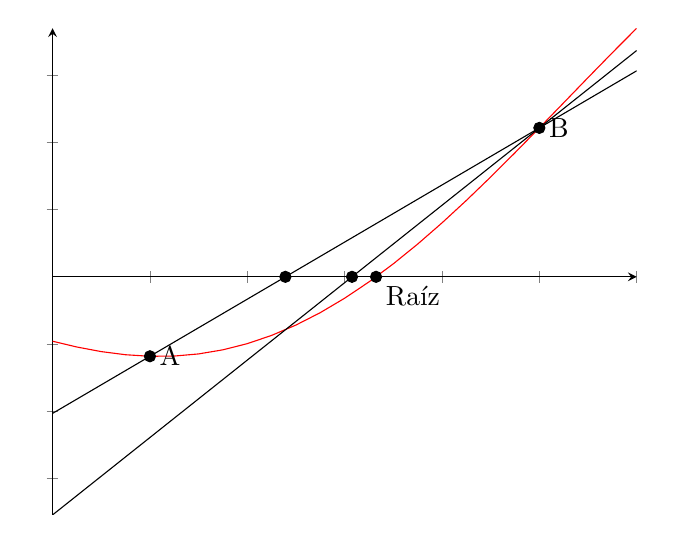
\begin{tikzpicture}
        \begin{axis}[
            axis x line = middle,
            axis y line =  center,
            grid = minor,
            xticklabels={,,},
            yticklabels={,,}
            ]
            \addplot[
                color = red,
                domain=0.5:3.5
                ]{x - 2*sin(deg(x)) - (1 / 2)};
            \addplot[
                color = black,
                domain=0.5:3.5
                ]{(((2.2177 - -1.1829) * (x - 1)) / (3 - 1)) + -1.1829};
            \addplot[
                color = black,
                domain=0.5:3.5
                ]{(((2.2177 - -0.788714) * (x - 1.6957)) / (3 - 1.6957)) + -0.788714};
            \filldraw[black] (2.1613,-0.0000037) circle (2pt) node[anchor=north west]{Raíz};
            \filldraw[black] (1, -1.1829) circle (2pt) node[anchor=west]{A};
            \filldraw[black] (3, 2.2177) circle (2pt) node[anchor=west]{B};
            \filldraw[black] (1.6957, 0) circle (2pt) node[anchor=west]{};
            \filldraw[black] (2.0378, 0) circle (2pt) node[anchor=west]{};
        \end{axis}
    \end{tikzpicture}
    \caption{Gráfica del método de la falsa posición}
    \label{regula_grap_ej1}
\end{figure}
\subsection{Deducción del método}

Originalmente en \cite{AN_Spanish}, tenemos que si se pueden elegir dos aproximaciones iniciales $ x_{n-1} $ y $ x_n $ tales que los dos valores de la función de esos puntos tengan signo opuesto en una función continúa comprendida entre $ [x_{n-1}, x_n] $ ], entonces es posible generar una sucesión de valores que siempre tengan esta propiedad.\newline\newline
Para iniciar, construimos la recta que pasa por los puntos $ (x_{n-1}, f(x_{n-1})) $ y $ (x_n, f(x_n) $. De acuerdo con la figura, se tiene que $ m_1 = m_2 $;\newline\newline

%Grafica

Se calcula la intersección con el eje $ x $ de la recta trazada anteriormente y a este punto se le denotará como $ x_{n+1} $.\newline\newline
Para encontrar la ecuación general que nos dará $ x_{n+1} $ en cada recta trazada, primero necesitamos encontrar la pendiente de la recta $ m_2 $:

\begin{displaymath}
    m_2 = \frac{f(x_n) - f(x_{n-1})}{x_n - x_{n-1}}
\end{displaymath}

Luego encontramos la pendiente de la recta $ m_1 $ que quedaría desde el intercepto hasta el extremo del intervalo en donde la función cambia de signo:

\begin{displaymath}
    m_1 = \frac{f(x_{n+1}) - f(x_{n-1})}{x_{n+1} - x_{n-1}}
\end{displaymath}

Por tanto, igualando las ecuaciones de ambas pendientes, debido que son dos segmentos de la misma recta:

\begin{displaymath}
    m_1 = m_2
\end{displaymath}

\begin{displaymath}
    \frac{f(x_{n+1}) - f(x_{n-1})}{x_{n+1} - x_{n-1}} = \frac{f(x_n) - f(x_{n-1})}{x_n - x_{n-1}}
\end{displaymath}

El valor del cruce por cero se define cuando se tiene un valor de $ x_{n+1} $, dado por la recta definida por la ecuación anterior, donde se cumple que $ f(x_{n+1}) = 0 $.\newline\newline
Así, la ecuación anterior queda de la siguiente forma:

\begin{displaymath}
    \frac{0 - f(x_{n-1})}{x_{n+1} - x_{n-1}} = \frac{f(x_n) - f(x_{n-1})}{x_n - x_{n-1}}
\end{displaymath}

Despejando $ x_{n+1} $ se obtiene:

\begin{displaymath}
    (x_n - x_{n-1})(0 - f(x_{n-1})) = (x_{n+1} - x_{n-1})(f(x_n) - f(x_{n-1}))
\end{displaymath}

\begin{displaymath}
    -\frac{(x_n - x_{n-1})(f(x_{n-1}))}{(f(x_n) - f(x_{n-1}))} = (x_{n+1} - x_{n-1})
\end{displaymath}

\begin{equation}
    \label{eq1_regula_falsi}
    x_{n+1} = x_{n-1} - \frac{(x_n - x_{n-1})(f(x_{n-1}))}{(f(x_n) - f(x_{n-1}))}
\end{equation}

Simplificando \eqref{eq1_regula_falsi}:

\begin{equation}
    \label{eq2_regula_falsi}
    x_{n+1} = \frac{(x_{n-1})(f(x_n)) - (x_n)(f(x_{n-1}))}{(f(x_n) - f(x_{n-1}))}
\end{equation}

Utilizando la ecuación \eqref{eq2_regula_falsi} anterior, el valor de $ x_{n+2} $ se elige tomando un valor entre $ x_{n-1} $ y $ x_n $ de tal forma que el valor de la función sea opuesto en signo a $ f(x_{n+1}) $. Así, valores de $ f(x_{n+1}) $ y $ x_{n+2} $ definen un menor intervalo que contiene el cruce por cero. El proceso continúa tomando siempre lados opuestos del cruce por cero. 
\section{Demostración de convergencia y análisis del error}

\subsection{Preliminares a tomar en cuenta \cite{MR_PDF}:}

Para la velocidad de convergencia, consideramos una secuencia $ [q_0,q_1,..] $ converge en $ q $, luego la diferencia $ (q_n - q) $ debe ser menor a medida que $ n $ se acerca al infinito; tomando la diferencia $ (q_n - q) $ como error $ (e_n) $, es dada por $ e_n = q_n - q $.\newline\newline
Tomando la proporción de errores sucesivos $ \frac{|e_{n+1}|}{|e_n|} $ queremos que sea menor que uno, es decir, si $ n $ tiende al infinito, la proporción debe ser menor que uno.

\begin{displaymath}
    \lim_{n^{-} \to \infty} (\frac{|e_{n+1}|}{|e_n|}) = k < 1
\end{displaymath}
	
Entonces el orden de convergencia es uno o la secuencia converge linealmente.\newline
Generalmente, tenemos:

\begin{displaymath}
    \lim_{n^{-} \to \infty} (\frac{|e_{n+1}|}{|e_n|^\alpha}) = k < 1
\end{displaymath}

\subsection{Tasa de convergencia:}

En el método de posición falsa, la secuencia de aproximación es $ {x_1,x_2,\ldots x_n} $ que converge en $ x $. Sea $ e_n $: el error se da como $ x_n - x $. La sucesión converge si $ |e_n| \rightarrow 0 $ como $ |n| \rightarrow \infty $. El orden de convergencia está determinado por una relación asintótica $ |e_n| $ y $ |e_n - 1| $. Ahora bien, si consideramos una función $ f(x)=0 $ en el intervalo $ (x_0, x_1) $ que contiene la raíz, luego en el método de posición falsa, uno de los dos puntos dados $ x_0 $ o $ x_1 $ siempre son fijos y otros varían. Si se fija el punto $ x_0 $, la función se aproxima mediante una recta que pasa por $ (x_0, f(x_0)) $ y $ (x_n, f(x_n)) $, donde $ n=1,2,\ldots $

% grafica

\subsection{Calcular el error:}

Sea $ {x_n} \rightarrow x $. Cuando $ x_n $ es una secuencia $ {x_0,x_1,x_2,\ldots} $ converge a $ x $, entonces el error en la iteración $ n_{th} $ es dado por $ e_n = x_n - x $ para $ n > 0 $.\newline\newline
Sea $ \lambda $ y $ \alpha $ constantes positivas tal que:

\begin{displaymath}
    \lim_{n^{-} \to \infty} (\frac{|x_{n+1} - x|}{|x_n - x|^\alpha})
\end{displaymath}

\begin{displaymath}
    \lim_{n^{-} \to \infty} (\frac{|e_{n+1}|}{|e_n|^\alpha}) = \lambda
\end{displaymath}

Sabemos por la formula de la falsa posición \eqref{eq2_regula_falsi}:

\begin{displaymath}
    x_{n+1} = \frac{(x_{n-1})(f(x_n)) - (x_n)(f(x_{n-1}))}{(f(x_n) - f(x_{n-1}))}
\end{displaymath}

Podemos reescribir la ecuación \eqref{eq2_regula_falsi} como:

\begin{equation}
    \label{eq3_regula_falsi}
    x_n = \frac{(x_{n-2})(f(x_{n-1})) - (x_{n-1})(f(x_{n-2}))}{(f(x_{n-1}) - f(x_{n-2}))}
\end{equation}

Además, calculamos sus errores como:

\begin{equation}
    \label{eq4_regula_falsi}
    e_n = x_n - x \rightarrow x_n = e_n + x
\end{equation}

\begin{equation}
    \label{eq5_regula_falsi}
    e_{n-1} = x_{n-1} - x \rightarrow x_{n-1} = e_{n-1} + x
\end{equation}

\begin{equation}
    \label{eq6_regula_falsi}
    e_{n-2} = x_{n-2} - x \rightarrow x_{n-2} = e_{n-2} + x
\end{equation}

Sustituyendo los valores de \eqref{eq4_regula_falsi}, \eqref{eq5_regula_falsi} y \eqref{eq6_regula_falsi} en la ecuación \eqref{eq3_regula_falsi} obtenemos:

\begin{displaymath}
    e_n + x = \frac{(e_{n-2} + x)(f(e_{n-1} + x))-(e_{n-1} + x)(f(e_{n-2} + x))}{f(e_{n-1} + x) - f(e_{n-2} + x)}
\end{displaymath}

\begin{displaymath}
    e_n = \frac{(e_{n-2} + x)(f(e_{n-1} + x))-(e_{n-1} + x)(f(e_{n-2} + x))}{f(e_{n-1} + x) - f(e_{n-2} + x)} - x
\end{displaymath}

Simplificando:

\begin{equation}
    \label{eq7_regula_falsi}
    e_n = \frac{(e_{n-2})(f(e_{n-1} + x))-(e_{n-1})(f(e_{n-2} + x))}{f(e_{n-1} + x) - f(e_{n-2} + x)}
\end{equation}

\subsection{Expandiendo por las series de Taylor:}

La expansión de Taylor es dada por:

\begin{displaymath}
    [f(a + h) = f(a) + hf^\prime(a) + \frac{h^2}{2}f^{\prime\prime}(a) + \ldots]
\end{displaymath}

Con ella obtenemos:

\begin{displaymath}
    \begin{split}
        &e_n - \frac{e_{n-2}[f(x) + e_{n-1}f^\prime (x) + (\frac{e_{n-1}^2}{2!}) f^{\prime\prime} (x) \ldots]}{[f(x) + e_{n-1}f^\prime (x) + \frac{e_{n-1}^2}{2! f^{\prime\prime} (x)}] - [f(x) + e_{n-2}f^\prime (x) + \frac{e_{n-2}^2}{2! f^{\prime\prime} (x)}]}\\
        &\quad - \frac{e_{n-1}[f(x) + e_{n-2}f^\prime (x) + (\frac{e_{n-2}^2}{2!}) f^{\prime\prime} (x) \ldots]}{[f(x) + e_{n-1}f^\prime (x) + \frac{e_{n-1}^2}{2! f^{\prime\prime} (x)}] - [f(x) + e_{n-2}f^\prime (x) + \frac{e_{n-2}^2}{2! f^{\prime\prime} (x)}]}
    \end{split}
\end{displaymath}

Efectuando:

\begin{displaymath}
    e_n = \frac{e_{n-1} e_{n-2}}{2} \frac{f^{\prime\prime} (x)}{f^\prime (x)}
\end{displaymath}

\begin{displaymath}
    e_n = \frac{1}{2} \frac{f^{\prime\prime} (x)}{f^\prime (x)} e_{n-1} e_{n-2}
\end{displaymath}

\begin{equation}
    \label{eq8_regula_falsi}
    e_n = C e_{n-1} e_{n-2}
\end{equation}

Donde $ C = \frac{1}{2} \frac{f^{\prime\prime} (x)}{f^\prime (x)} $ es la constante del error asintótico.\newline

Debido que Falsa posición se fija a un punto, por ejempo, podemos asumir $ Ce_{n-2} $ es una constante $ K $, por lo tanto, podemos reescribir \eqref{eq8_regula_falsi} como:

\begin{equation}
    \label{eq9_regula_falsi}
    e_n = K e_{n-1}
\end{equation}

Por lo tanto, de la ecuación \eqref{eq9_regula_falsi} se puede deducir que la falsa posición tiene una tasa de convergencia lineal cuando $ |K| < 1 $.
\section{Ventajas y Desventajas del método}

\subsection{Ventajas}

\begin{itemize}
    \item Es un método horquillado \footnote{Los métodos de horquillado determinan intervalos cada vez más pequeños (horquillas) que contienen una raíz.} y siempre es convergente.
    \item El error es controlable, a mayor número de iteraciones la raíz es más precisa.
    \item No requiere el cálculo de derivadas.
    \item No es necesario tener información de la función, aparte del signo de las imágenes.

\end{itemize}

\subsection{Desventajas}

\begin{itemize}
    \item La tasa de convergencia es lenta.
    \item Tiene una tasa de convergencia lineal.
    \item No logra determinar raíces complejas.
    \item No logra identificar múltiples raíces diferentes.
    \item No se puede aplicar en un intervalo donde la función toma valores del mismo signo.

\end{itemize}
\section{Pseudocódigo}

Para encontrar una solución para $ f(x) = 0 $ dada la función $ f $ continua en el intervalo $ (p_0, p_1) $ donde $ f(p_0) $ y $ f(p_1) $ tienen signos opuestos:

\begin{algorithm}
    \caption{Método de posición falsa}
    \KwIn{Aproximación inicial $ p_0, p_1 $;  tolerancia $ TOL $;  máximo número de iteraciones $ N_0 $.}
    \KwOut{Solución aproximada $ p $ o mensaje de error.}
    
    $ i = 2 $; $ q_0 = f(p_0) $; $ q_1 = f(p_1) $
    
    \BlankLine
    
    \While {$i \le N_0 $} {
        $ p = p_0 - \frac{q_0 (p_1 - p_0)}{q_1 - q_0} $
        
        \BlankLine
        
        \If{$ |p - p_0| < TOL $} {
                \tcp {Procedimiento exitoso}
                \KwOut {$ p $}
            }
        
        \BlankLine
        
        $ i = i + 1 $; $ q = f(p) $
        \BlankLine
        
        \If{$ q . q_1 < 0 $} {
                $ p_0 = p_1 $; $ q_0 = q_1 $
            }
            
        \BlankLine
        
        $ p_0 = p $; $ q_0 = q $
    }
    
    \KwOut{El método falló luego de $ N_0 $ iteraciones}
\end{algorithm}
\section{Ejemplos}

\subsection{Dato curioso}
El método de la falsa posición se aplica a la predicción de cantidades traza de contaminantes atmosféricos producidos por reacciones de combustión, como las que se encuentran en fuentes puntuales industriales.

\subsection{Ejercicio}
Considerando la función:
\begin{displaymath}
    f(x) = 1 + 2x - 3x^2e^{-x} + 2x^3sin(x)e^{- \frac{x}{5}}
\end{displaymath}
Calcular el cruce por cero dentro del intervalo $ [6, 7] $; usando un error máximo de $ 10^{–5} $.

\begin{table}[h!]
    \centering
    \caption{Resultados del cálculo de los cruces por cero.}
    \label{table1_regula_falsi}
    \begin{tabular}{c|c|c|c|c|c|c}
        \textbf{$ n $} & \textbf{$ x_{n-1} $} & \textbf{$ f(x_{n-1}) $} & \textbf{$ x_n $} & \textbf{$ f(x_n) $} & \textbf{$ x_{n+1} $} & \textbf{$ f(x_{n+1}) $}\\
        \hline
         $ 0 $ & $ 6.0000 $ & $ -23.624 $ & $ 7.0000 $ & $ 126.00 $ & $ 6.1578 $ & $ -3.9574 $ \\
         $ 1 $ & $ 6.1578 $ & $ -3.9574 $ & $ 7.0000 $ & $ 126.00 $ & $ 6.1835 $ & $ -0.5292 $ \\ 
         $ 2 $ & $ 6.1835 $ & $ -0.5292 $ & $ 7.0000 $ & $ 126.00 $ & $ 6.1869 $ & $ -0.0681 $ \\ 
         $ 3 $ & $ 6.1869 $ & $ -0.0681 $ & $ 7.0000 $ & $ 126.00 $ & $ 6.1873 $ & $ -0.0087 $ \\ 
         $ 4 $ & $ 6.1873 $ & $ -0.0087 $ & $ 7.0000 $ & $ 126.00 $ & $ 6.1874 $ & $ -0.0011 $ \\ 
         $ 5 $ & $ 6.1874 $ & $ -0.0011 $ & $ 7.0000 $ & $ 126.00 $ & $ 6.1874 $ & $ -0.0001 $ \\ 
         $ 6 $ & $ 6.1874 $ & $ -0.0001 $ & $ 7.0000 $ & $ 126.00 $ & $ 6.1874 $ & $ -1.8e-5 $ \\ 
    \end{tabular}
\end{table}

El cruce por cero de la función $ f(x) $ en $ [6, 7] $ nos devuelve un valor de $ x_{n+1} = 6.1874$

\begin{figure}[!ht]
    \centering
    \begin{tikzpicture}
        \begin{axis}[
            axis x line = middle,
            axis y line =  center,
            grid = minor
            ]
            \addplot[
                color = red,
                domain = 5:10
                ]{1 + 2*x - 3*(x^2)*pow(e,-x) + 2*(x^3)*sin(deg(x))*pow(e,-x/5)};
            \filldraw[black] (6.1874, -0.000018) circle (2pt) node[anchor=south west]{$ (6.1874, -0.000018) $};
        \end{axis}
    \end{tikzpicture}
    \caption{Gráfica de $ f(x) = 1 + 2x - 3x^2e^{-x} + 2x^3sin(x)e^{- \frac{x}{5}} $}
    \label{regula_grap_ej2}
\end{figure}
\clearpage
\section{Método de Muller.}
\section{Introducción al método de Muller.}
Originalmente en \cite{muller1956method} se planteó un método para encontrar raíces de funciones algebraicas
a través de un procedimiento iterativo que consiste en utilizar un polinomio interpolante de segundo 
grado para encontrar su raíz más cercana al valor de la ecuación que se quiere resolver. Partiendo de dicha premisa es que
a continuación se presenta una deducción y análisis del método, sin embargo, primero es necesario definir algunos preliminares
matemáticos que serán útiles para justificar argumentos hechos posteriormente y en consecuencia presentar el método en su totalidad.
\subsubsection{Preliminares matemáticos.}
\subsubsection{Polinomio interpolante.}
Si se conoce el valor de una función $f(x)$ en n+1 puntos defínase el polinomio
interpolante como un polinomio de grado n que pasa por los n+1 puntos
previamente establecidos y se utiliza para aproximar los valores de $f(x)$ en las cercanías de cada punto.
La deducción más detallada de cómo se puede encontrar dicho polinomio y toda la teoría detrás
se salen del ámbito de esta investigación, sin embargo, una explicación puede encontrarse en cualquier texto
sobre análisis y métodos numéricos (véase por ejemplo \cite{atkinson}).
\subsubsection{Polinomio interpolante de Newton.}
\begin{definition}
    \label{newton_poly}
    Dado un conjunto distinto de puntos $(x_n,f(x_n)),\ldots,(x_0,f(x_0))$ se define
    el polinomio interpolante de Newton como un polinomio de grado n de la forma
    \begin{equation}
        \begin{split}
            &P(x) =f[x_n]+f[x_n,x_{n-1}](x-x_n)\\
            &\quad +f[x_n,x_{n-1},x_{n-2}](x-x_n)(x-x_{n-1})\\
            &\qquad + \cdots + f[x_n,\ldots,x_0](x-x_n)(x-x_{n-1})\cdots(x-x_1) 
        \end{split} 
    \end{equation}  
\end{definition}
donde $f[x_n,\ldots,x_i]$ es la operación conocida como diferencia dividida de Newton,
la cual se definirá más adelante. Del anterior planteamiento es posible observar cómo
los n+1 puntos acaban definiendo un polinomio de grado n que sirve para interpolar
la función en los valores conocidos.
\subsubsection{Cota de error de un polinomio interpolante}
Considerando entonces que un polinomio interpolante aproxima una función 
en las cercanías de los n+1 puntos que lo definen, es posible estimar cuál es
la magnitud máxima del error que se comente al realizar tal aproximación. Sea $P(x)$ el
polinomio interpolante y $f(x)$ una función con n+1 derivadas continuas definidas en el menor intervalo $I$ que contenga los números reales $[x_n,x_{n-1},\ldots,x_0]$,
se define el error cometido como la expresión
\begin{equation}
    \label{lagrange_error}
    f(x)-P(x)=\frac{f^{\left(n+1\right)}(\xi)}{(n+1)!}(x-x_n)\cdots(x-x_0)
\end{equation}
con $\xi \in I$. \\De nuevo la demostración de la anterior expresión
va más allá del ámbito de este trabajo y puede encontrarse en cualquier
libro de análisis numérico.
\subsubsection{Diferencias divididas.}
Dada una función $f(x)$ se definen sus diferencias divididas como una
operación recursiva de la forma
\begin{align*}
    f[x_n]                      &= f(x_n)\\
    f[x_n,x_{n-1}]              &= \frac{f[x_{n-1}]-f[x_n]}{x_{n-1}-x_n}\\
                                &\phantom{=} \vdots\\
    \numberthis \label{newton_div}f[x_n,\ldots,x_0] &= \frac{f[x_{n-1},\ldots,x_0]-f[x_{n},\ldots,x_1]}{x_0-x_n} 
\end{align*}
Donde $f[x_n,x_{n-1}]$ es la primera diferencia dividida, $f[x_n,x_{n-1},x_{n-2}]$
es la segunda diferencia dividida y así sucesivamente.

\begin{lemma}
    \label{diff_deriv}
    $f[x_n,\ldots,x_0]=\frac{f^n(\xi)}{n!}$ para algún $\xi \in I$, donde $I$ es el intervalo
    más pequeño que contiene los números reales $[x_n,\ldots,x_0]$.
    \begin{proof}
        Primero se plantea una función $f(x) \in C^nI$ aproximada por un polinomio interpolante
        $P(x)$ de grado n partiendo de n+1 puntos $[x_n,\ldots,x_0]$ establecido anteriormente
        en la definición (\ref{newton_poly}). Dado que $P(x)$ es una interpolación de $f(x)$ se plantea la
        función $g(x)=f(x)-P(x)$ la cual tiene n+1 raíces, así que por el teorema de Rolle
        generalizado se tiene que:
            \begin{equation}
                \begin{split}
                    g^n(\xi)&=f^n(\xi)-P^n(\xi)=0\\
                    g^n(\xi)&=f^n(\xi)-f[x_n,\ldots,x_0]n!=0\\
                    f[x_n,\ldots,x_0] &= \frac{f^n(\xi)}{n!}
                \end{split}
            \end{equation}
    \end{proof}
\end{lemma}
\section{Deducción del método.}
Para encontrar alguna raíz de la función algebraica $f(x)$ primero 
se parte de tres puntos $\bigl\{\bigl(x_2,f(x_2)\bigr),\bigl(x_1,f(x_1)\bigr),\bigl(x_0,f(x_0)\bigr)\bigr\}$ que sirven como base para 
encontrar un polinomio interpolante de segundo grado que aproxime la función
$f(x)$. Sin perder generalidad se asume que $x_2<x_1<x_0$ y se define $w(x)=x-x_2$, por lo
que el polinomio interpolante tiene la forma
\begin{equation}
    \label{quatraic_muller}
    P(w)=aw^2+bw+c
\end{equation}
El motivo de esto es que se quiere encontrar el valor más pequeño $x-x_2$ que sea al mismo tiempo
una raíz del polinomio así que lo planteado en \ref{quatraic_muller} simplifica ligeramente
el álgebra a desarrollar para encontrar los valores buscados en la ecuación.\\

De lo anterior entonces es necesario encontrar los valores de $a,b,c$
para saber cuál es el polinomio interpolante en los puntos establecido,
para esto se plantea el siguiente sistema de ecuaciones
\begin{align}
    \label{eq1_muller}P(w(x_2))&=c=f(x_2)\\
    \label{eq2_muller}P(w(x_1))&=a(x_1-x_2)^2+b(x_1-x_2)+f(x_2)=f(x_1)\\
    \label{eq3_muller}P(w(x_0))&=a(x_0-x_2)^2+b(x_0-x_2)+f(x_2)=f(x_0)
\end{align}
Sustrayendo \ref{eq2_muller} de \ref{eq3_muller}
\begin{multline*}
    a\Bigl((x_0-x_2)^2-(x_1-x_2)^2\Bigr)+b\Bigl((x_0-x_2)-(x_1-x_2)\Bigr)\\=f(x_0)-f(x_1)
\end{multline*}
\begin{multline*}
    a\Bigl[\Bigl((x_0-x_2)-(x_1-x_2)\Bigr)\Bigl((x_0-x_2)+(x_1-x_2)\Bigr)\Bigr]\\
    +b\Bigl((x_0-x_2)-(x_1-x_2)\Bigr)=f(x_0)-f(x_1)
\end{multline*}
\begin{multline*}
    a\Bigl[(x_0-x_2)+(x_1-x_2)\Bigr]+b=\frac{f(x_0)-f(x_1)}{(x_0-x_2)-(x_1-x_2)}
\end{multline*}
\begin{equation*}
    a\Bigl[(x_0-x_2)+(x_1-x_2)\Bigr]+b=\frac{f(x_0)-f(x_1)}{x_0-x_1}
\end{equation*}
\begin{equation*}
    a\Bigl[(x_0-x_2)+(x_1-x_2)\Bigr]+b=f[x_0,x_1]
\end{equation*}
\begin{equation}
    \label{eq4_muller}
    b=f[x_0,x_1]-a\Bigl[(x_0-x_2)+(x_1-x_2)\Bigr]
\end{equation}
Ahora sustituyendo \refeq{eq4_muller} en \refeq{eq2_muller}
\begin{multline*}
    a(x_1-x_2)^2+\Bigl(f[x_0,x_1]-a(x_0+x_1+2x_2)\Bigr)(x_1-x_2)\\
    +f(x_2)=f(x_1)
\end{multline*}
\begin{multline*}
    a(x_1-x_2)^2-a(x_0+x_1-2x_2)(x_1-x_2)+f[x_0,x_1](x_1-x_2)\\
    +f(x_2)=f(x_1)
\end{multline*}
\begin{multline*}
    a\Bigl((x_1-x_2)(x_1-x_2-x_0-x_1+2x_2)\Bigr)+f[x_0,x_1](x_1-x_2)\\+f(x_2)=f(x_1)
\end{multline*}
\begin{equation*}
    a\Bigl((x_1-x_2)(x_2-x_0)\Bigr)+f[x_0,x_1](x_1,x_2)+f(x_2)=f(x_1)
\end{equation*}
\begin{equation*}
    a(x_2-x_0)+f[x_0,x_1]=\frac{f(x_1)-f(x_2)}{x_1-x_2}
\end{equation*}
\begin{equation*}
    a(x_2-x_0)=f[x_1,x_2]-f[x_0,x_2]
\end{equation*}
\begin{equation}
    \label{eq5_muller}
    a=\frac{f[x_1,x_2]-f[x_0,x_1]}{x_2-x_0}=f[x_2,x_1,x_0]
\end{equation}
Sustituyendo \refeq{eq5_muller} en \refeq{eq4_muller}
\begin{equation*}
    b=f[x_0,x_1]-f[x_2,x_1,x_0]\Bigl[(x_0-x_2)+(x_1-x_2)\Bigr]
\end{equation*}
\begin{equation*}
    b=f[x_0,x_1]-f[x_2,x_1,x_0](x_0-x_2)-f[x_2,x_1,x_0](x_1-x_2)
\end{equation*}
\begin{equation*}
    b=f[x_0,x_1]-f[x_0,x_1]+f[x_2,x_1]-f[x_2,x_1,x_0](x_1-x_2)
\end{equation*}
\begin{equation*}
    b=f[x_2,x_1]+f[x_2,x_1,x_0](x_2-x_1)
\end{equation*}
\begin{equation*}
    b=f[x_2,x_1]+\frac{(x_1-x_2)\frac{\bigl(f(x_0)-f(x_1)\bigr)}{x_0-x_1}+(x_1-x_2)\left(\frac{f(x_1)-f(x_2)}{x_1-x_2}\right)}{x_0-x_2}
\end{equation*}
\begin{multline*}
    b=f[x_2,x_1]+\frac{\frac{x_2-x_1}{x_0-x_1}\bigl(f(x_0)-f(x_1)\bigr)+f(x_1)-f(x_2)}{x_0-x_2}\\
    -\frac{f(x_0)-f(x_2)}{x_0-x_2}+f[x_2,x_0]
\end{multline*}
\begin{multline*}
    b=f[x_2,x_1]+f[x_2,x_0]\\
    +\frac{\frac{x_2-x_1}{x_0-x_1}\bigl(f(x_0)-f(x_1)\bigr)+f(x_1)-f(x_2)-f(x_0)+f(x_2)}{x_0-x_2}
\end{multline*}
\begin{multline*}
    b=f[x_2,x_1]+f[x_2,x_0]\\
    +\frac{\frac{x_2-x_1}{x_0-x_1}\bigl(f(x_0)-f(x_1)\bigr)-f(x_0-f(x_1))}{x_0-x_2}
\end{multline*}
\begin{equation*}
    b=f[x_2,x_1]+f[x_2,x_0]+\frac{\bigl(f(x_0)-f(x_1)\bigr)\left(\frac{x_2-x_1}{x_0-x_1}-1\right)}{x_0-x_2}
\end{equation*}
\begin{equation*}
    b=f[x_2,x_1]+f[x_2,x_0]+\frac{\bigl(f(x_0)-f(x_1)\bigr)\left(\frac{x_2-x_1-x_0+x_1}{x_0-x_1}\right)}{x_0-x_2}
\end{equation*}
\begin{equation*}
    b=f[x_2,x_1]+f[x_2,x_0]+\frac{\bigl(f(x_0)-f(x_1)\bigr)\left(\frac{x_2-x_0}{x_0-x_1}\right)}{x_0-x_2}
\end{equation*}
\begin{equation*}
    b=f[x_2,x_1]+f[x_2,_x0]-\frac{f(x_0-f(x_1))}{x_0-x_1}\frac{x_0-x_2}{x_0-x_2}
\end{equation*}
\begin{equation}
    \label{eq6_muller}
    b=f[x_2,x_1]+f[x_2,x_0]-f[x_1,x_0]
\end{equation}
Con los planteamientos anteriores entonces sabemos que
\begin{equation*}
    a=f[x_2,x_1,x_0]
\end{equation*}
\begin{equation*}
    b=f[x_2,x_1]+f[x_2,x_0]-f[x_1,x_0]
\end{equation*}
\begin{equation*}
    c=f(x_2)
\end{equation*}
lo cual significa que se tienen los datos suficientes para despejar (\refeq{quatraic_muller})
y encontrar $w$, así que utilizando la fórmula cuadrática se tiene que
\begin{equation*}
    w=\frac{-b\pm\sqrt{b^2-4ac}}{2a}=-\frac{2c}{b\pm\sqrt{b^2-4ac}}
\end{equation*}
y haciendo las sustituciones correspondientes se puede concluir entonces que
\begin{equation*}
    x=x_2-\frac{2f(x_2)}{b\pm\sqrt{b^2-4f(x_2)f[x_2,x_1,x_0]}}
\end{equation*}
aplicando de forma sucesiva la ecuación anterior se tiene
\begin{equation}
    \label{muller_algorithm}
    x_{n+1}=x_n-\frac{2f(x_n)}{b\pm\sqrt{b^2-4f(x_n)f[x_n,x_{n-1},x_{n-2}]}}
\end{equation}
lo cual concluye la deducción del método de Muller para encontrar
raíces de funciones algebraicas.
\section{Análisis de convergencia.}
\subsection{Demostración de convergencia.}
Sea $p$ la raíz de la función $f(x)$ que se busca encontrar con el algoritmo,
se asume que si $x_n \rightarrow p$ entonces por el lemma \refeq{diff_deriv} $b \rightarrow f'(p)$
y $a \rightarrow f''(p)$ entonces sustituyendo en (\refeq{muller_algorithm}) se tiene que
\begin{equation}
    \label{muller_convergence_eq}
    p = p - \frac{2f(p)}{f'(p)\pm\sqrt{\left(f'(p)\right)^2-4f(p)f''(p)}}
\end{equation}
y ya que por definición $f(p)=0$ se puede concluir que la expresión (\refeq{muller_convergence_eq})
es igual a $0$ siempre que $f'(p) \neq 0$ así que el método converge a una raíz de la ecuación.
\subsection{Análisis del error y orden de convergencia.}
Para establecer una expresión que defina el error del método anteriormente planteado se define $P(p)$
como el polinomio interpolante de segundo grado evaluado en la raíz $p$ y $f(p)$ como la función aproximada
evaluada en su raíz. Además por (\refeq{muller_algorithm}) se sabe que $x_{n+1}$ es una raíz del polinomio
interpolante, entonces por (\ref{lagrange_error}) se sabe que
\begin{equation}
    \label{error_muller_eq1}
    P(p)-f(p)=-\frac{f'''(\xi)}{6}(p-x_n)(p-x_{n-1})(p-x_{n-2})
\end{equation}
luego $f(p)=0$ y utilizando el teorema del valor medio se sabe que 
\[\frac{P(p)-P(x_{n+1})}{p-x_{n+1}}=f'(p),\,P(p)=f'(p)(p-x_{n+1})\]
ya que $P(x_{n+1})=0$, entonces sustituyendo en (\refeq{error_muller_eq1}) se tiene
\begin{equation}
    \label{error_muller_eq2}
    p-x_{n+1}=-\frac{f'''(p)}{6f'(p)}(p-x_n)(p-x_{n-1})(p-x_{n-2})
\end{equation}
lo cual es un punto de partida suficiente para establecer el error del método y 
posteriormente su orden de convergencia. Utilizando la notación de error $|e_{n+1}|=|p-x_{n+1}|$
y definiendo $M=|\frac{f'''(p)}{6f'(p)}|$ se puede reescribir \refeq{error_muller_eq2} como
\begin{equation}
    \label{error_muller}
    |e_{n+1}|=M|e_{n}||e_{n-1}||e_{n-2}|
\end{equation}
y utilizando la definición de orden de convergencia se tiene que
\begin{equation}
    \label{error_e0}
    |e_{n+1}|=C|e_n|^\alpha
\end{equation}
lo cual implica también que
\begin{equation}
    \label{error_e1}
    |e_n|=C|e_{n-1}|^\alpha
\end{equation}
y despejando $|e_{n-1}|$ se tiene
\begin{equation}
    \label{error_e2}
    |e_{n-1}|=\left(\frac{1}{C}|e_n|\right)^\frac{1}{\alpha}
\end{equation}
y de forma similar 
\[|e_{n-1}|=C|e_{n-2}|^\alpha\]
así que sustituyendo la ecuación anterior en (\refeq{error_e2}) y despejando $|e_{n-2}|$ se tiene
\begin{equation}
    \label{error_e3}
    |e_{n-2}|=\frac{1}{C^{\frac{1}{\alpha}+\frac{1}{\alpha^2}}}|e_n|^{\frac{1}{\alpha^2}}
\end{equation}
por lo que reemplazando (\refeq{error_e0}), (\refeq{error_e1}), (\refeq{error_e2}) y (\refeq{error_e3})
en (\refeq{error_muller}) se tiene que
\begin{equation*}
    C|e_n|^\alpha=M|e_n|\frac{1}{C^{\frac{1}{\alpha}}}|e_n|^{\frac{1}{\alpha}}\left(\frac{1}{C^{\frac{1}{\alpha}+\frac{1}{\alpha^2}}}\right)|e_n|^{\frac{1}{\alpha^2}}
\end{equation*}
simplificando entonces se tiene que
\begin{equation}
    \label{muller_order_eq}
    C|e_n|^\alpha=\frac{M}{C^{\frac{2}{\alpha}+\frac{1}{\alpha^2}}}|e_n|^{1+\frac{1}{\alpha}+\frac{1}{\alpha^2}}
\end{equation}
lo cual implica que $C=\frac{M}{C^{\frac{2}{\alpha}+\frac{1}{\alpha^2}}}$ y $\alpha=1+\frac{1}{\alpha}+\frac{1}{\alpha^2}$
por lo que despejando $\alpha$ se llega a la ecuación $\alpha^3-\alpha^2-\alpha-1=0$ de la que resolviendo se
sabe entonces que $\alpha \approx 1.84$, lo cual indica que el orden de convergencia del método de Muller es aproximadamente
1.84: menor que el método de Newton pero mejor que bisección por ejemplo. Sabiendo entonces su orden de convergencia se tiene que
\[|p-x_1|=C|p-x_0|^{1.84}\]
\[C^{0.84}|p-x_1|=\left(C|p-x_0|\right)^{1.84}\]
y de forma inductiva se tiene que
\begin{equation}
    \label{x_0_convergence}
    C^{0.84}|p-x_{n+1}|=(C|p-x_0|)^{1.84^{n}}
\end{equation}
entonces se debe cumplir que $C|p-x_0|<1$ para que posteriormente cuando $n\rightarrow\infty,\, x_n\rightarrow p$. En otras palabras,
la convergencia del método está garantizada únicamente si el punto inicial escogido está lo suficientemente cerca de la raíz a encontrar.
\subsection{Ventajas y desventajas.}
\subsubsection{Ventajas.}
\begin{itemize}
    \item Su convergencia es bastante rápida, siendo considerablemente mejor que métodos como bisección.
    \item Permite encontrar no solo raíces reales sino también complejas.
    \item No requiere el cálculo de ninguna derivada para su implementación.
\end{itemize}
\subsubsection{Desventajas.}
\begin{itemize}
    \item Se necesita conocer un valor cercano a la raíz que se desea encontrar.
    \item Puede resultar en raíces complejas incluso si solo se buscan raíces reales.
    \item No es posible garantizar convergencia si la raíz está en un punto crítico (véase \refeq{muller_convergence_eq}).
\end{itemize}
\subsection{Pseudocódigo.}
El siguiente algoritmo asume la utilización de aritmética de números complejos dentro del mismo,
además la operación de diferencias divididas calculada de forma externa con un procedimiento similar
al mostrado en (\refeq{newton_div}). La condición de paro es que el valor absoluto de la función evaluada
en la última aproximación encontrada sea menor a una tolerancia $\epsilon$ o que la cantidad de iteraciones
supere un valor límite previamente establecido.
\begin{algorithm}
    \DontPrintSemicolon
    \KwData{$x_2,x_1,x_0$ valores distintos para interpolar $f(x)$, un valor $\epsilon$ de tolerancia y un valor $N$
    que define la cantidad máxima de iteraciones.}
    \KwResult{La raíz de $f(x)$ más cercana a los puntos iniciales dados o un mensaje de error en
    caso de que no se cumpla la tolerancia mínima}
    \Begin{
    $x_{n+1} \gets 0$\;
    $x_{n} \gets x_2$\;
    $x_{n-1} \gets x_1$\;
    $x_{n-2} \gets x_0$\;
    $x_{n+1} \gets 3$\;
    \While{$|f(x_{n+1})|<\epsilon \,{\bf or}\, i \geq N $}{
        $a \gets f[x_n,x_{n-1},x_{n-2}]$\;
        $b \gets f[x_n,x_{n-1}]+f[x_n,x_{n-2}]-f[x_{n-1},x_{n-2}]$\;
        $c \gets f(x_n)$\;
        $D \gets \sqrt{b^2-4ac}$\;
        \tcc{Escoge el valor de mayor magnitud para el denominador}
        \eIf(){$|b-D|\le|b+D|$}{
            $E \gets b+D$
        }(){$E \gets b-d$}
        $x_{n+1} \gets x_n-\frac{2c}{E}$\;
        $x_{n-2} \gets x_{n-1}$\;
        $x_{n-1} \gets x_{n}$\;
        $x_{n} \gets x_{n+1}$\;
        $i \gets i+1$
    }
    \eIf{$|f(x_{n+1})|<\epsilon$}{
        \Return{$x_{n+1}$}
    }
    {\KwOut{No se pudo encontrar un valor para la raíz.}}
    }
    \caption{Método de Muller\label{IR}}
\end{algorithm}
\subsection{Ejemplos.}
\subsubsection{Visualizando algunas iteraciones}
Como primer ejemplo para visualizar el algoritmo se puede utilizar el polinomio deducido en
(\refeq{muller_order_eq}) y encontrar todas sus raíces haciendo uso del algoritmo. Primero se presenta
una gráfica del polinomio como función compleja, representando en los ejes $x,y$ de la gráfica el plano
complejo y en el eje $z$ de la gráfica el módulo de cada valor de la función, tal representación resulta útil para visualizar
dónde se encuentran las raíces en el plano complejo. Las tres raíces del polinomio con seis decimales 
correctos son: 
\begin{align*}
    \left(+1.839286+0.000000i\right)\\(-0.419643-0.606290i)\\(-0.419643+0.606290i)
\end{align*}
Una gráfica de dicho polinomio puede verse en la figura \refeq{zero_poly} (con $z$ siendo un número complejo).
Se consideran algunas iteraciones del método de Muller con su respectiva forma y sus raíces de modo que se pueda visualizar
su comportamiento y sucesiva aproximación a una de las raíces. Eligiendo los puntos más cercanos a cada raíz
es posible utilizar el método para encontrarlas todas.\\
\begin{figure}
    \centering
    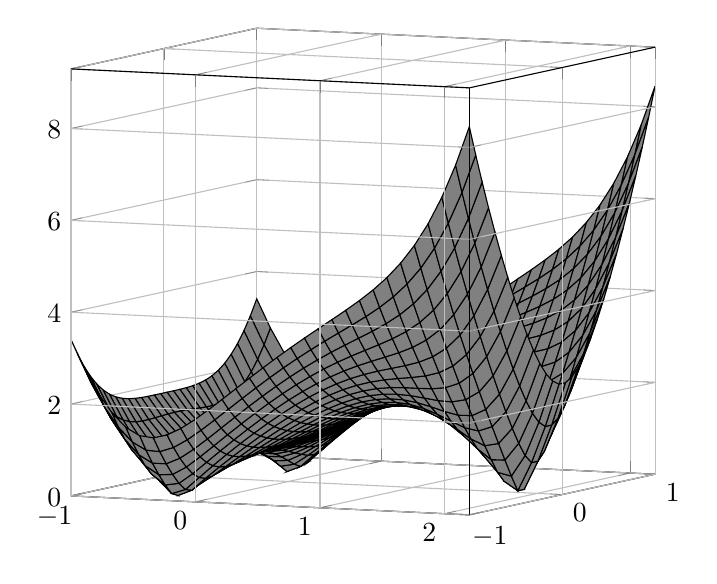
\begin{tikzpicture}
        \begin{axis}[view={25}{6},zmin=0,grid,
            3d box = complete*]
        \addplot3 [
            domain=-1:2.2,
            domain y = -1:1,
            samples = 30,
            samples y = 30,
            surf,
            fill=black!50,
            faceted color=black] {((3*x^2*y-2*x*y-y^3-y)^2+(x^3-x^2-3*x*y^2-x+y^2-1)^2)^(1/2)-0.2};
        \end{axis}
    \end{tikzpicture}
    \caption{Polinomio $z^3-z^2-z-1$}
    \label{zero_poly}
\end{figure} 
\begin{figure}
    \centering
    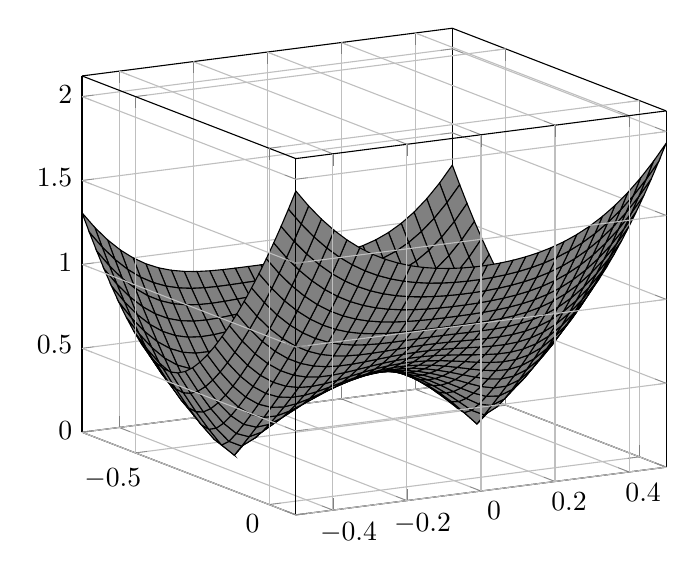
\begin{tikzpicture}
        \begin{axis}[view={60}{15},zmin=0,grid,
            3d box = complete*]
        \addplot3 [
            domain=-0.7:0.1,
            domain y = -0.5:0.5,
            samples = 30,
            samples y = 30,
            surf,
            fill=black!50,
            faceted color=black] {((-4*((x+2)^2-y^2)+13*(x+2)-11)^2+(13*y-8*(x+2)*y)^2)^(1/2)};
        \end{axis}
    \end{tikzpicture}
    \caption{Primera iteración}
    \label{first_poly}
\end{figure}
\begin{figure}
    \centering
    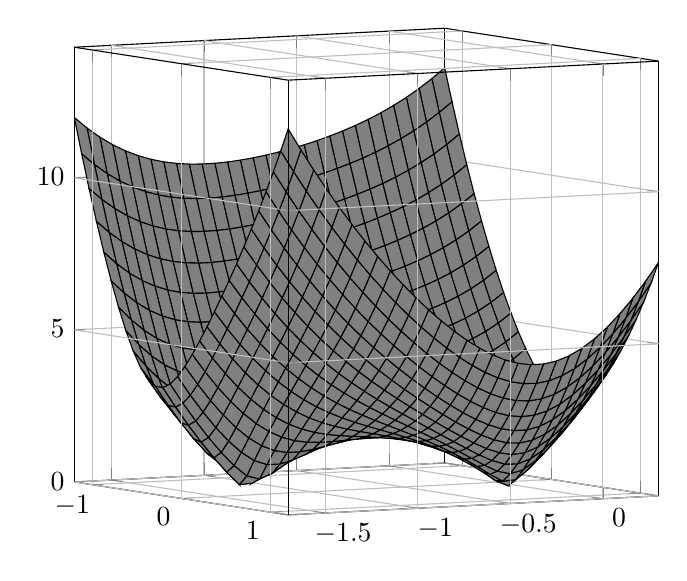
\begin{tikzpicture}
        \begin{axis}[view={60}{5},zmin=0,grid,
            3d box = complete*]
        \addplot3 [
            domain=-1.2:1.2,
            domain y = -1.7:0.3,
            samples = 30,
            samples y = 30,
            surf,
            fill=black!50,
            faceted color=black] {((0.330719*x^2-8.75*x*y-5.2915*x-0.330719*y^2+1.57092)^2+(-4.375*x^2-0.661438*x*y+2*x+4.375*y^2+5.2915*y+0.46875)^2)^(1/2)};
        \end{axis}
    \end{tikzpicture}
    \caption{Segunda iteración}
    \label{second_poly}
\end{figure}
\begin{figure}
    \centering
    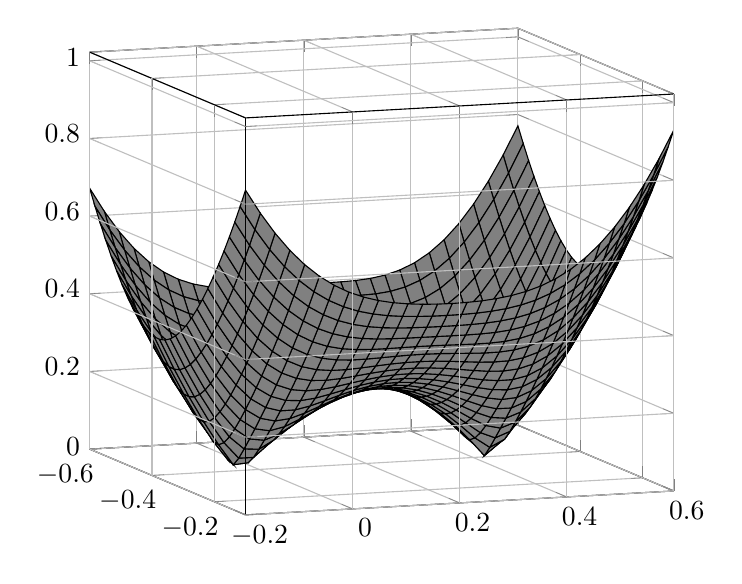
\begin{tikzpicture}
        \begin{axis}[view={70}{10},zmin=0,grid,
            3d box = complete*]
         
        \addplot3 [
            domain=-0.6:-0.1,
            domain y = -0.2:0.6,
            samples = 30,
            samples y = 30,
            surf,
            fill=black!50,
            faceted color=black] {((0.844055*x^2-7.59798*x*y+2.0208*x-0.844055*y^2-2.58721*y+0.665431)^2+(-3.79899*x^2-1.68811*x*y-2.58721*x+3.79899*y^2-2.0208*y-0.511867)^2)^(1/2)};
        \end{axis}
    \end{tikzpicture}
    \caption{Tercera iteración}
    \label{third_poly}
\end{figure}
\begin{table}[h!]
    \centering
    \caption{iteraciones del método.}
    \label{iterations_table}
    \begin{tabular}{c|c|c}
        \textbf{Iteración} & \textbf{Raíz 1} & \textbf{Raíz 2}\\
        \hline
        1 & $+1.625000+0.330718i$ & $+1.625000-0.330718i$\\
        2 & $+0.219445-1.020150i$ & $+0.326009-0.148102i$\\
        3 & $-0.381386-0.049646i$ & $-0.380227+0.412363i$\\
    \end{tabular}
\end{table}
\newpage
El cuadro \ref{iterations_table} muestra las sucesivas aproximaciones de las raíces de los polinomios interpolantes
hacia la tercera raíz de la función original $(-0.419643+0.606290i)$, siendo que con únicamente tres iteraciones la
magnitud de la distancia de la raíz más cercana del tercer polinomio interpolante y la raíz de la función original es
de tan solo $0.197892$. Dos iteraciones más garantizan que $|f(x_n)<\epsilon|$ si se asume $\epsilon=10^{-6}$.
\clearpage
\section{Método de Newton-Raphson en $\mathbb{C}$}
\section{Introducción al método}

Encontrar raíces de polinomios ha sido una tarea de suma importancia más allá del ámbito de la matemática teórica, pues tiene múltiples aplicaciones desde gráficas de computadora, como puede verse en¨\cite{3b1b} hasta resolución de problemas de optimización. Su relevancia es aún mayor cuando teorías como las de Galois y el teorema de Abel Ruffini limitan las fórmulas que directamente permiten la obtención de sus raíces \cite{badger} más allá de polinomios de grado 4.
Es por esto, que la creación de algoritmos o herramientas que puedan resolver dichas limitantes, son muy importantes para el ámbito matemático; ahora no solo su existencia es necesaria, si no que se desea que estas sean lo más rápidas y eficaces posibles. 

Entre estos resalta el método descubierto por Isaac Newton y luego refinado por Joseph Rahpson, el cual permite encontrar aproximaciones a las raíces de polinomios con una gran rapidez mediante pocas iteraciones y con un gran precisión al mismo tiempo. Veremos ahora porque se da esto y como funciona el método de Newton y como se puede extender más allá de los reales
\section{Demostración del método}
Supongamos que $ f \in C^2[a,b] $ y sea $ p_n \in [a,b]$ una aproximación a \textit{p} de tal forma que $f'(p_n) \neq 0$ y $ | p - p_n | $ es un valor pequeño. Encontrando el primer polinomio de Taylor para $f(x)$ en $p_n$ y evaluado en $x = p$, se obtiene:

\begin{displaymath}
 f(p) = f(p_n) + (p-p_n)f'(p_n) + \frac{(p-p_o)^2}{2!}f''(\xi(p))
\end{displaymath}


\noindent Donde $\xi(p)$ es un valor que se encuentra entre $p$ y $p_n$. Dado que $f(p) = 0$, se obtiene lo siguiente

\begin{displaymath}
 0 = f(p_n) + (p-p_n)f'(p_n) + \frac{(p-p_n)^2}{2!}f''(p)
\end{displaymath}


Como asumimos que $ | p - p_n | $ es un valor pequeño, entonces el valor obtenido de $(p-p_n)^2$ es aún más pequeño, lo que permite que sea despreciable, quedando así la ecuación como

\begin{displaymath}
    0 \approx f(p_n) + (x-p_n)f'(p_n)
\end{displaymath}

resolviendo para \textit{p} obtenemos

\begin{displaymath}
    p \approx p_n - \frac{f(P_n)}{f'(p_n)}
\end{displaymath}

De lo cual obtenemos el método de Newton-Raphson, el cual a partir de un punto inicial $p_0$ se obtiene una sucesión $\{p\}^\infty_{n=0}$ y una aproximación a la raíz \textit{p}

\begin{equation}
    p = p_{n-1} - \frac{f(p_{n-1})}{f'(p_{n-1})}
\end{equation}

Obteniendo asi mismo una ecuación que será muy útil para encontrar el error y demostrar convergencia de Newton-Raphson
\begin{displaymath}
0 = \frac{f(p_n)}{f'(p_n)} + p-p_o +(x-p_n)^2 \frac{f''(p)}{2!f'(p)}
\end{displaymath}
\begin{displaymath}
p = p_n - \frac{f(p_n)}{f'(p_n)}  - (p-p_n)^2 \frac{f''(p)}{2!f'(p)}
\end{displaymath}
\begin{displaymath}
p = p_{n+1}  - (p-p_n)^2 \frac{f''(p)}{2!f'(p)}
\end{displaymath}
\begin{displaymath}
p - p_{n+1} =  - (p-p_n)^2 \frac{f''(p)}{2!f'(p)}
\end{displaymath}
\subsection{Convergencia del método de Newton-Raphson}

El método de Newton tiene una convergencia considerablemente rápida, permitiendo obtener una aproximación extremadamente precisa con pocas iteraciones, como puede verse en ejemplo 1, y puede intuirse a través de su derivación por medio de series de Taylor, donde se asume que $ | p - p_o | $ es un valor pequeño, lo que permite desechar su elevación cuadrática $(p-p_o)^2$.

Sin embargo, esto representa una limitante para el método, que requiere que la aproximación inicial $p_0$ se encuentre lo bastante cerca del valor real de \textit{p} para poder cumplir dicha asunción. Si este es el caso y se cumple que $f'(p) \neq 0$ entonces el método de Newton garantiza su convergencia, como puede verse en el siguiente teorema

\begin{theorem}
Sea $f \in C^2[a,b]$ con \textit{f} continua en $[a,b]$ y $p \in (a,b)$, y con $f(p) = 0$ y $f'(x) \neq 0$ y siendo $f,f', f''$ continuas, existe entonces un $\delta > 0$  tal que Newton - Raphson genera una sucesión $\{p\}^\infty_{n=0}$ que converge a p para cualquier valor inicial tomado de $[p-\delta, p+\delta]$.
\end{theorem}

\begin{proof}
Partiendo que Newton-Raphson es un esquema de iteración proveniente de punto fijo\cite{atkinson}, pues $p = g(p_{n-1}), n \geq 0$ y obteniendo de él la sucesión $\{p\}^\infty_{n=0}$, para que esta converja, dada la existencia de un  $\delta > 0$, debe existir un $\epsilon$ tal que $|p - x| < \epsilon$ para toda x en  $[p-\delta, p+\delta]$.

Sea 
\begin{displaymath}
M = \frac{Max_{x}|f''(x)|}{Min_{x}|f'(x)|}
\end{displaymath}

de la deducción del polinomio de Taylor para el método de newton, tenemos que 
\begin{displaymath}
 p - p_n = - (p-p_n)^2\frac{f'(p_n)}{2f''(p_n)}
\end{displaymath}
De esto, obtenemos que 
\begin{displaymath}
| p - p_{n+1}| \leq M|p - p_n|^2
\end{displaymath}
\begin{displaymath}
M| p - p_{n+1}| \leq (M|p - p_n|)^2
\end{displaymath}

Siendo $[p-\delta, p+\delta]$ un sub-intervalo dentro de $[a,b]$ y partiendo de la existencia de un $\delta$, implica la existencia de un $\epsilon$ tal que $| p - p_0| \leq \epsilon$  y tomando que $M| p - p_0| < 1$. Teniendo también que $M| p - p_1| < 1$ y $M| p - p_1| < M| p - p_0|$, que implica $| p - p_1| \leq \epsilon$ y por transitividad, podemos extender el argumento hasta $p_n$ valores mediante inducción demostrando que  $| p - p_n| \leq \epsilon$  y  $M| p - p_n| < 1$ para $n \geq 0$

\begin{displaymath}
M| p - p_{n}| \leq (M|p - p_0|)^2
\end{displaymath}
\begin{displaymath}
| p - p_{n}| \leq \frac{1}{M}(M|p - p_0|)^2
\end{displaymath}

como $(M|p - p_0|)^2 < 1$ entonces 
\begin{displaymath}
\lim_{n->\infty}{| p - p_{n}|} = \lim_{n->\infty}{\frac{1}{M}}
\end{displaymath}


En base a lo anterior y demostrando también a través de la definición de limites para sucesiones, siendo $L = 0$ y habiendo comprobado la existencia de $\epsilon$, se concluye que

\begin{displaymath}
\lim_{p->\infty}{\{p\}^\infty_{n=0}} = 0
\end{displaymath}

y por lo tanto el método de Newton-Raphson converge para cualquier valor $p_0$ tomado dentro del intervalo $[p-\delta, p+\delta]$.

\end{proof}

\subsection{Convergencia para dos raíces o más}

Habiendo observado como el método de Newton converge de manera muy rápida hacia la raíz cuando existe solamente una, podemos extender la anterior definición para emplear el método a n raíces, con $n \geq 2$, partiendo de la premisa que todo $p_0$ dentro de $[p-\delta, p+\delta]$ convergerá al valor de la raíz más cercana, siempre y cuando dentro del intervalo escogido se cumplan las condiciones de que $f,f'$ son continuas y $f'(p_0) \neq 0$, y por lo tanto podemos enunciar la siguiente definición

\begin{definition}

Si $p_*$ es una raíz de \textit{f}, el área de atracción de $p_*$ esta compuesta por todos aquellos valores $p_0$ tales que el método de Newton al comenzar desde $p_0$ converge hacia $p_*$

\begin{displaymath}
B(x_*) = {x_0|x_n =  N^n(x_0) \xrightarrow{}  x_*}
\end{displaymath}

\end{definition}

A partir de la determinación del tipo de puntos al que pertenecen los valores de $p_0$, podremos establecer que los puntos iniciales tenderán a la raíz más cercana. 
Los tipos de puntos fijos se establecen en base a la siguiente definición:

\begin{definition}
 Supóngase un mapa $f: X \xrightarrow[]{}X$ es diferenciable en un punto fijo $p_*$, entonces
 \begin{itemize}
     \item $p_*$ es atrayente si y solo si $|f(p_*)|<1$
     \item $p_*$ es super-atrayente si y solo si $|f(p_*)|=0$
     \item $p_*$ es repelente si y solo si $|f(p_*)|>1$
 \end{itemize}
\end{definition}

Entonces, en vista de que $|g'(p)| = 0$ ya que 
\begin{displaymath}
     g(x)= 1 - \frac{f(x)}{f'(x)} 
\end{displaymath}

con derivada 

\begin{displaymath}
     g'(x)= 1 - \frac{(f'(x)f'(x))-(f(x)f''(x))}{(f'(x))^2} = \frac{(f(x)f''(x))}{(f'(x))^2}
\end{displaymath}

y asumiendo que $f(p)=0$
\begin{displaymath}
     g'(x)= 0
\end{displaymath}

lo que permite concluir que los puntos dentro del intervalo $[p-\delta, p+\delta]$, son super-atrayentes y por ende convergerán a la raíz más cercana

Este comportamiento puede observarse buscando las raíces de la ecuación $x^2-1 = 0$, la cual posee dos raíces reales 1 y -1 como puede verse en Figura \ref{fig:graph_cuadratica}. 

\begin{figure}[H]
    \begin{tikzpicture}
\begin{axis}[
axis x line = middle,
axis y line =  center,
grid = minor
]
\addplot[
color=red,
]{x^2-1};
\addplot[only marks] table {
1   0
-1  0
};
\end{axis}
\end{tikzpicture}
\centering
    \caption{Gráfica de $x^2-1$}
    \label{fig:graph_cuadratica}
\end{figure}


Coloreando cada $p_0$ en base a que raíz se acercarán en la aproximación, vemos que obtenemos la siguiente imagen

Donde se observa como el plano se divide en dos partes uniformes con su respectivo color, en base a cual será la raíz a la que el valor se aproximará

\begin{figure}[h]
    \centering
    
\includegraphics{images/eq1-1.png}
    \caption{Zonas de convergencia de $x^2-1$}
    \label{fig:eq_cuadratica_1}
\end{figure}

si, ahondamos más en la imagen y generamos un gradiente de color, donde mientras más oscuro más rápidamente converge el punto, o lo que es lo mismo, menos iteraciones se necesitan, obtenemos lo siguiente:
\begin{figure}[H]
    \centering
    
\includegraphics[scale=0.26]{images/eq1-2.png}
    \caption{Rapidez de convergencia de los puntos de $x^2-1$}
    \label{fig:eq_cuadratica_2}
\end{figure}


Donde podemos ver que al aproximarnos a 0, los ritmos de convergencia tienden a aumentar de manera drástica, al punto de no converger.
Esto se debe a que si evaluamos un valor de $p_n = 0$, $g'(0) = 2x = 2(0) = 0$, indefiniendo el resultado del método en ese punto

Veamos otro ejemplo con un comportamiento curioso, el cual también tiene puntos donde el método se indefine
Sea $f(x) = x^3-x$, que al resolver algebraicamente obtenemos $(x-1)(x-0)(x+1)$ con raices en 1,0,-1.
A partir de su gráfica vemos que existen dos puntos críticos, que determinándolos a través de $f'(x) = 0$ da como resultado $-\frac{1}{\sqrt{3}}, \frac{1}{\sqrt{3}}$. 

\begin{figure}[h]
    \begin{tikzpicture}
\begin{axis}[
axis x line = middle,
axis y line =  center,
grid = minor
]
\addplot[
color=red,
]{x^3-x};
\addplot[only marks] table {
1   0
-1  0
0   0
};
\end{axis}
\end{tikzpicture}
\centering
    \caption{Gráfica de $x^3-x$}
    \label{fig:graph_cubica}
\end{figure}


De esto podemos concluir que $(-\infty,-\frac{1}{\sqrt{3}}) \subset  B(-1)$ y $(\frac{1}{\sqrt{3}}, \infty) \subset  B(1)$. Para el caso de $B(0)$, su determinación es un poco más complicada, ya que debemos tomar en cuenta los puntos crítico, los cuales producirán un efecto cíclico, en este caso de período 2, en Newton-Raphson si se les tome como puntos iniciales o cualquier punto inicial que, después de n iteraciones, haga que la tangente de la función sea igual a uno de ellos \cite{wiersma}. 

Partiendo la premisa anterior premisa, tenemos que determinar en que punto $x_0 = x_2$, es decir $x = N(N(x)) = N^2(x)$.  Este proceso se simplifica ya que $f$ es una función impar y entonces $-f(x) = f(-x)$, por lo tanto a través de simetría tenemos que obtendremos $N^2(x)$ si $-x = N(x)$. Para esto calculamos la función en el método

\begin{gather*}
    N(x) = x - \frac{x^3-x}{3x^2-1} \\
    N(x) = \frac{2x^3}{3x^2-1}
\end{gather*}

luego igualamos a -x y resolvemos

\begin{gather*}
    -x = \frac{2x^3}{3x^2-1}\\
    0 = 5x^3-x\\
    x = \pm \frac{1}{\sqrt{5}} \vee x = 0
\end{gather*}

Y de esto podemos concluir que $(-\frac{1}{\sqrt{5}},\frac{1}{\sqrt{5}}) \subset B(0)$
\\
\\
Ahora bien, veamos que pasa entre los valores de $(-\frac{1}{\sqrt{3}},-\frac{1}{\sqrt{5}})$ y $(\frac{1}{\sqrt{5}},\frac{1}{\sqrt{3}})$. Como la función es simétrica, entonces lo que pasa en $(\frac{1}{\sqrt{5}},\frac{1}{\sqrt{3}})$, será igual que en $(-\frac{1}{\sqrt{3}},-\frac{1}{\sqrt{5}})$. En estos dos intervalos se suceden áreas de convergencia hacia $B(1)$ y $B(-1)$, las cuales se ven divididas por valores los cuales luego de n iteraciones caerían en alguno de los puntos críticos de la función, indefiniendo el método.



Veamos por ejemplo un punto un poco a la izquierda de $\frac{1}{\sqrt{3}}$, por ejemplo 0.5773442692, el cual si evaluamos en Newton, nos devolverá $-18518.03739$, un valor que se encuentra dentro de los puntos convergentes hacia -1, hasta que encontremos un valor cuya n iteración sea $-\frac{1}{\sqrt{3}}$ , el cual al igualar ese valor en el método obtenemos 0.465601, por lo tanto $(\frac{1}{\sqrt{3}},0.465601) \subset  B(-1)$.
Si luego probamos con 0.465600, la siguiente iteración devuelve un número positivo muy grande, que cae dentro de $B(1)$. Este comportamiento se mantendrá hasta que hallemos un número cuya n-esima iteración de como resultado $\frac{1}{\sqrt{3}}$ e indefina la función. 

Estos patrones continúan y se alternan entre cada división causada por valores que iteren hacia alguno de los puntos críticos de la función, y podremos determinar cada una de estas divisiones igualando l a función a uno de los puntos previos obtenidos,, esto nos genera unos patrones curiosos, como puede verse en Figura \ref{fig:eq_cubica_1} y \ref{fig:eq_cubica_2}
\begin{figure}[H]

        \centering
        
\includegraphics{images/eq2-1.png}
        \caption{Áreas de convergencia de $x^3-x$}
        \label{fig:eq_cubica_1}
\end{figure}
    
\begin{figure}[H]
    \centering
    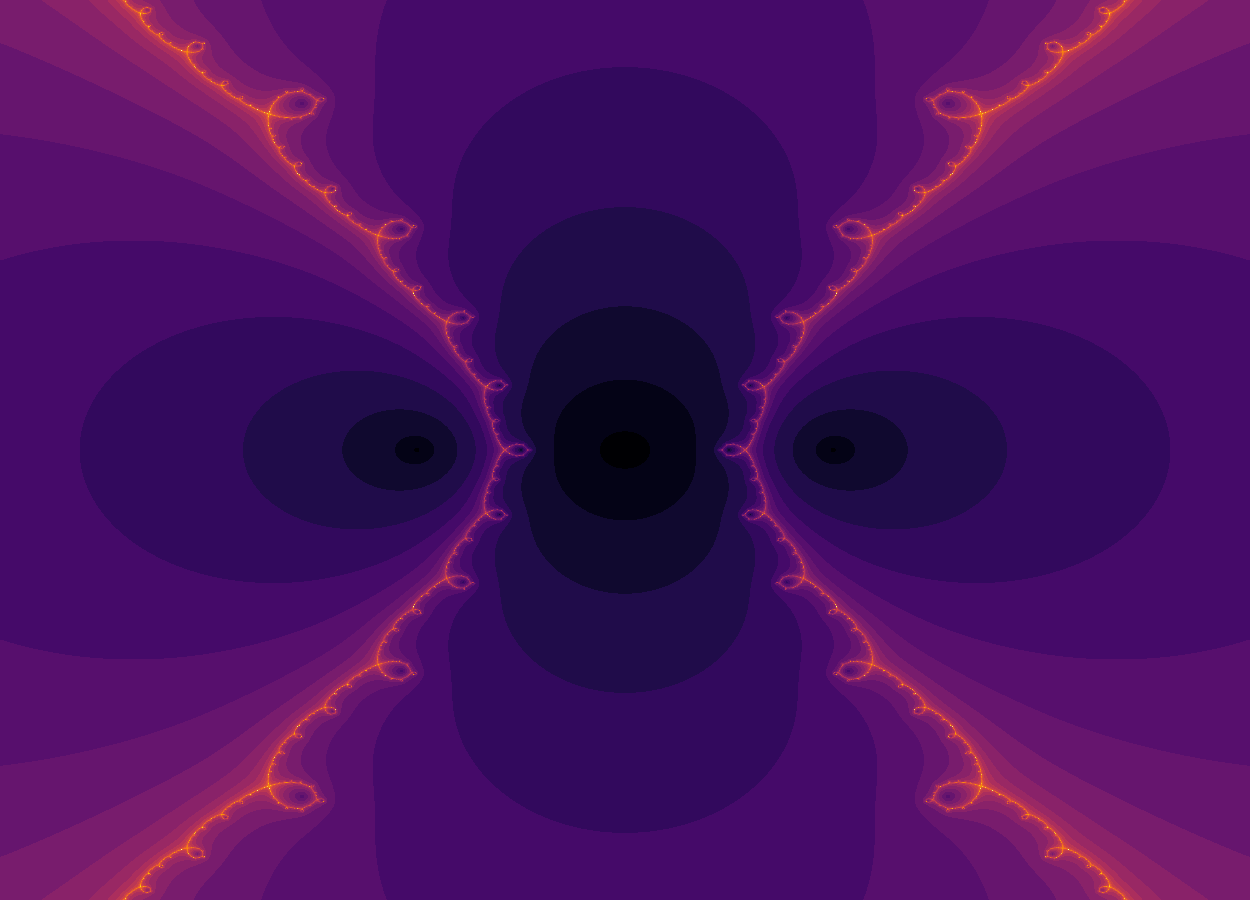
\includegraphics[scale=0.26]{images/eq2-2.png}
    \caption{Rapidez de convergencia de los puntos de $ x^3-x$}
    \label{fig:eq_cubica_2}
\end{figure}

\section{Análisis del error del método de Newton-Raphson}

El error del método de Newton, puede obtenerse a partir de su deducción del método de Taylor, donde 
\begin{displaymath}
p - p_{n+1} =  - (p-p_n)^2 \frac{f''(p)}{2!f'(p)}
\end{displaymath}

es el error obtenido a través de la aproximación polinomial. 
Sin embargo, mediante el Teorema del Valor Medio, puede obtenerse una fórmula más sencilla para obtener el error a lo largo de las iteraciones del método

\begin{displaymath}
f(p_n)= f(p_n) - f(p) = f'(\xi)(p_n-p)
\end{displaymath}
\begin{displaymath}
\frac{f(p_n)}{ f'(\xi)} =(p_n-p)
\end{displaymath}

Donde si $f'(\xi)$ no cambia rápidamente entre p y $p_n$, entonces $f'(\xi) = f'(p)$ y
\begin{displaymath}
(p_n-p)= \frac{f(p_n)}{ f'(\xi)} = p_{n+1} - p_n
\end{displaymath}
obteniendo así la fórmula del error estándar de Newton
\begin{equation}
(p_n-p)=  p_{n+1} - p_n
\end{equation}
\subsection{Análisis sobre la eficiencia del método de Newton-Raphson}

El método de Newton-Raphson, tiene una convergencia cuádratica, como se demostrará partiendo del siguiente teorema

\begin{theorem}
Asumiendo que $f,f',f''  $sean continuas para toda x en las proximidades de $p$ y asumiendo que $f(p) = 0, f'(p) \neq 0 $.Entonces si se escoge lo suficientemente cerca de $p$ , las iteraciones del método de Newton Raphson convergen a $p$. Con un orden de convergencia cuadrático
\end{theorem}

\begin{proof}
Partiendo de 

\begin{displaymath}
\lim_{n->\infty}{\frac{p_{n+1} - p}{p_n - p}} = \lambda
\end{displaymath}
Usaremos el polinomio de Taylor de $f(x)$ en \textit{p}
\begin{displaymath}
 0 = f(p_n) + (p-p_n)f'(p_n) + \frac{(p-p_n)^2}{2}f''(p)
\end{displaymath}
obtenemos
\begin{displaymath}
p - p_{n+1} =  - (p-p_n)^2 \frac{f''(p)}{2f'(p)}
\end{displaymath}
\begin{displaymath}
\frac{|p - p_{n+1}|}{|(p-p_n)^2|} = \frac{f''(p)}{2f'(p)}
\end{displaymath}

\begin{displaymath}
\lim_{n->\infty}{\frac{|p - p_{n+1}|}{|(p-p_n=|)^2}} =  \frac{f''(p)}{2f'(p)}
\end{displaymath}
Lo que prueba que la convergencia del método es cuadrática
\end{proof}


\section{Extensión del método al Dominio de $\mathbb{C}$}

El teorema fundamental del álgebra enuncia lo siguiente:

\begin{theorem}
 Todo polinomio de grado n $n \geq 1$ tiene n raíces complejas
\end{theorem}

Cuya demostración se puede encontrar en \cite{lankham}

A partir de esto, podemos expandir la búsqueda de raíces incluyendo números imaginarios y pasar del plano exclusivamente real, al plano complejo  $\mathbb{C}$ y extender a su vez el método de Newton-Raphson, cuya única modificación será que ahora es capaz de recibir funciones complejas y puntos iniciales del mismo tipo

\begin{equation}
     z = z_{n-1} - \frac{f(z_{n-1})}{f'(z_{n-1})}
\end{equation}

Por ejemplo, sea $f(z) = z^2+1, f'(z) = 2z$, veremos que obtenemos las  raíces $-i,i$ con la siguiente imagen de sus puntos de convergencia
\begin{figure}[H]
    \centering
    
\includegraphics{images/eq3-1.png}
    \caption{ Zonas de convergencia de $ x^2+1$}
    \label{fig:eq_cuad_compleja_1}
\end{figure}

y si colocamos el mapa de la rapidez de convergencia de sus puntos (Los colores más claros indican mayor cantidad de iteraciones)
\begin{figure}[H]
    \centering
    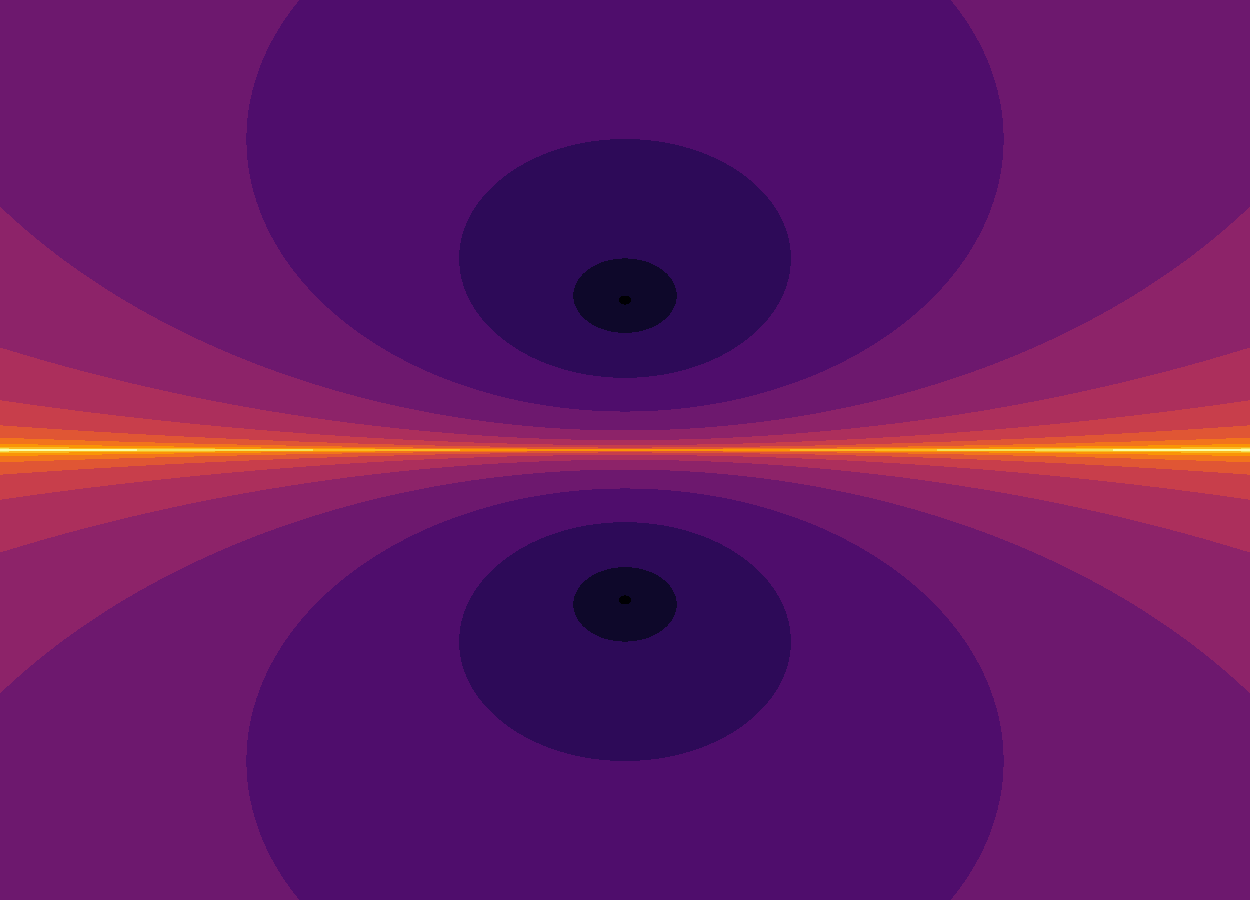
\includegraphics[scale=0.26]{images/eq3-2.png}
    \caption{Rapidez de convergencia de los puntos de $ x^2+1$}
    \label{fig:eq_cuad_compleja_2}
\end{figure}
Comportándose muy similar a la función vista previamente en Figura \ref{fig:eq_cuadratica_2}, con la división siendo en este caso el eje de los reales 

Pero que pasa con funciones de grado $n \geq 2$
Si observamos la función $f(z) = z^3-1$, obtenemos las raíces $(-0.5,-0.866i),(-0.5+0.866i),(1+0i)$ y al generar su mapa de convergencia, obtenemos la siguiente imagen, la cual genera un patrón interesante
\begin{figure}[H]
    \centering
    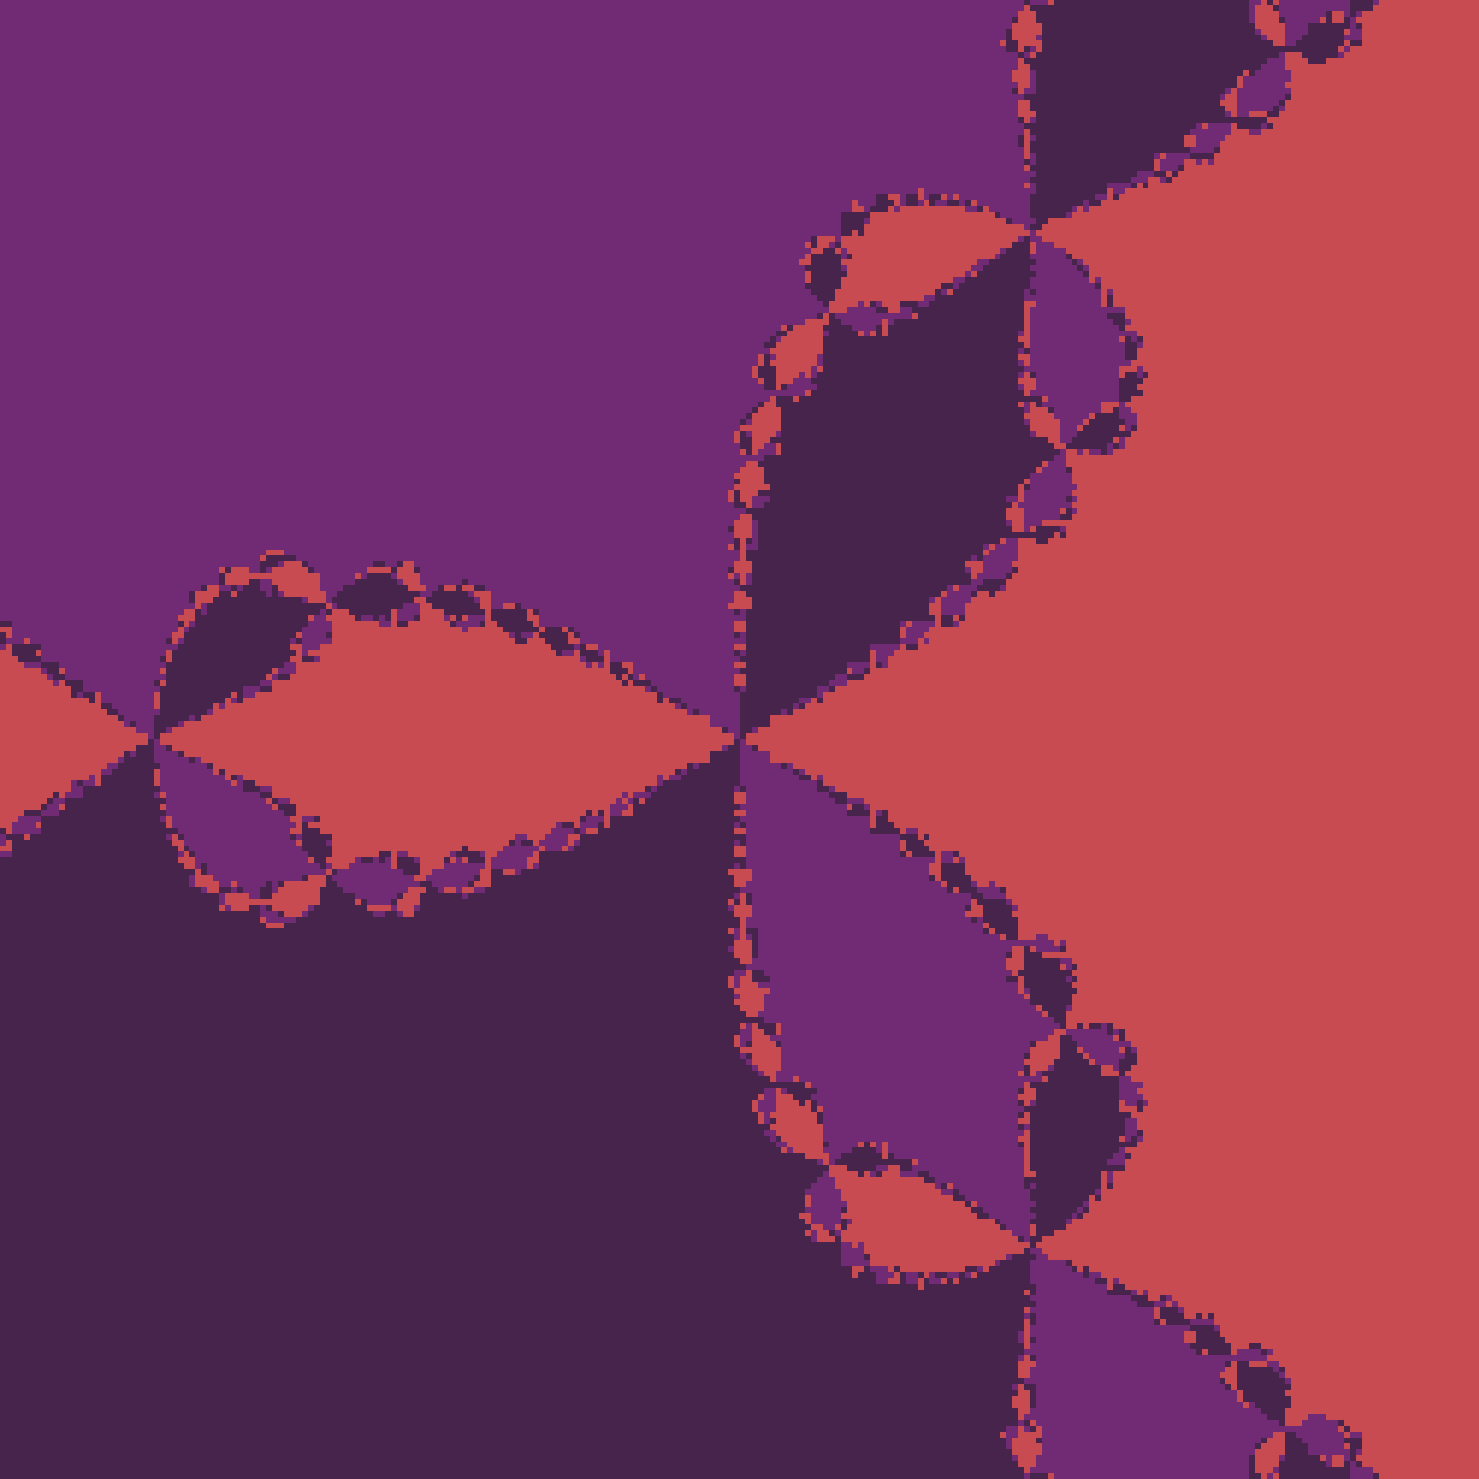
\includegraphics{images/eq4-1.png}
    \caption{Zonas de convergencia de los puntos de $ x^3-1$}
    \label{fig:eq_cub_compleja_1}
\end{figure}
y si se gráfica de la rapidez de convergencia de sus puntos vemos lo siguiente
\begin{figure}[H]
    \centering
    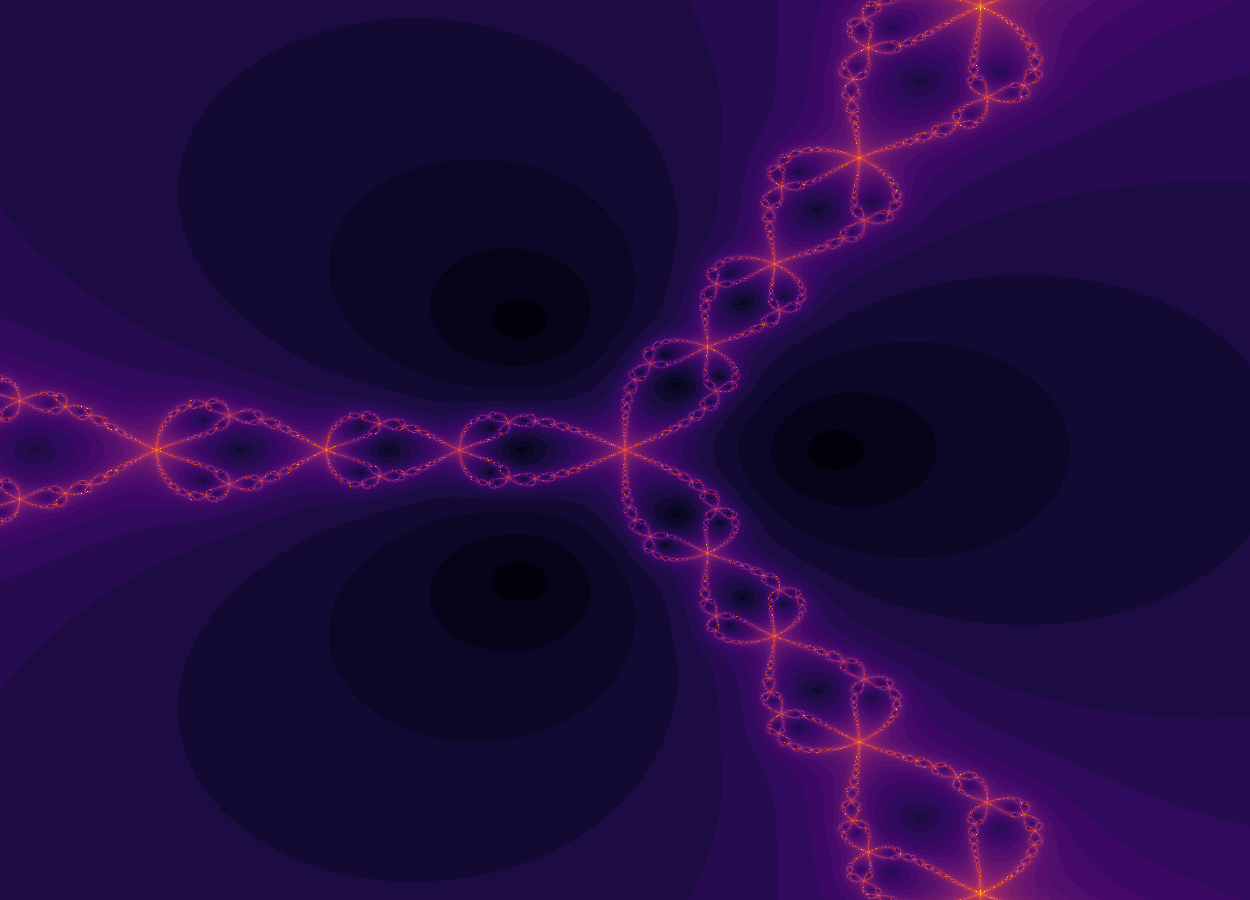
\includegraphics[scale=0.26]{images/eq4-2.png}
    \caption{Rapidez de convergencia de los puntos de $ x^3-1$}
    \label{fig:eq_cub_compleja_2}
\end{figure}
Aquí notamos dos comportamientos inusuales
El primero de ellos es que se forma un fractal muy similar a un conjunto de Julia\cite{badger}, y que se empezaba a vislumbrar en la Figura \ref{fig:eq_cuadratica_2}, donde cerca de los bordes donde comenzaría la siguiente región de otra raíz, observamos una formación que, sin importar el nivel de acercamiento que se le de, contiene colores correspondientes a otras zonas de atracción, los cuales a su vez contienen más de estas zonas de atracción de las demás raíces. Estos fractales son conocidos como fractales de Newton \cite{3b1b}

Podemos ver en esto que se réplica la idea de que entre regiones donde el método tomaría muchas iteraciones o donde fallase, se ven contenidas zonas de atracción hacia las demás raíces, pero además podemos observar que cada zona es dividida entre lugares donde todos los puntos convergen hacia una única raíz o lugares donde se contienen n colores divididos de manera recursiva en estas dos zonas

Además se puede apreciar, como ya se mencionaba, que existen zonas, cerca de los bordes y de los puntos críticos, donde los valores de puntos iniciales tomados de dicho sitio tomarán una gran cantidad de iteraciones en converger, como puede verse en \ref{fig:eq_cubica_1}, extendiendo el comportamiento visto dentro de los reales con al función $x^3-x$.

Dichos comportamientos pueden verse en funciones de mayor grado, como puede verse en los ejemplos ilustrados de la sección correspondiente
\section{Ventajas y desventajas del método }

\subsection{Ventajas}

\begin{itemize}
    \item Tiene una rápida convergencia al ser cuadrático
    \item Requiere pocas iteraciones para obtener una alta precisión en el valor de la aproximación
    \item Requiere únicamente un punto inicial
    \item El método es muy fácil de implementar si se cumplen las condiciones que le validan
\end{itemize}

\subsection{Desventajas}

\begin{itemize}
    \item La aproximación inicial debe de estar lo bastante cercana a \textit{p} como para que se cumpla la  condición de que $( p - p_o )^2$ es descartable, caso contrario el método de Newton puede nunca converger independientemente del número de iteraciones \cite{burden}
    \item $f'$ debe de ser continua y debe de conocerse, de lo contrario el método no puede ser aplicado
    \item Si existe algún máximo o mínimo dentro del intervalo de interés, el método no converge
\end{itemize}
\section{Pseudocódigo}
\begin{algorithm}
\SetKwComment{Comment}{/* }{ */}

\caption{Método de Newton-Raphson en $\mathbb{C}$ }
\KwIn{aproximación inicial $z_0$, tolerancia TOL, máximo número de iteraciones $n_{max}$}\
\KwOut{solución aproximada a  \textit{p} o mensaje de error}
$ i = 1$ 
\BlankLine
$z = z_0 - f(z_0)/f'(z_0)$
\BlankLine
\While{$i \le n_max $}{
    \If{$\|z-z_0\|<TOL$}{\tcp{Procedimiento exitoso}\Return{z}} 
    $i = i + 1$
    \BlankLine
    $z = z_0$
}
\Return \KwOut{"El metodo fallo luego de N iteraciones, N="$n_{max}$}
\end{algorithm}

\setcounter{subsection}{0}
\section{Ejemplos} 
Encuentre  las raíces de los siguientes polinomios utilizando Newton-Rahpson y muestre el gradiente de convergencia de la función:


\textbf{Función:}$x^7-x-1$

\textbf{Raíces:}

\begin{center}
\begin{tabular}{ c c }
 (-0.8099-0.2629i) & (-0.8099+0.2629i) \\
 (-0.3636-0.9526i) & (-0.3636+0.9526i) \\
 (0.6171-0.9009i) & (0.6171-0.9009i) \\  
 (1.1128-0i)  
\end{tabular}
\end{center}


\begin{figure}[H]
    \centering
    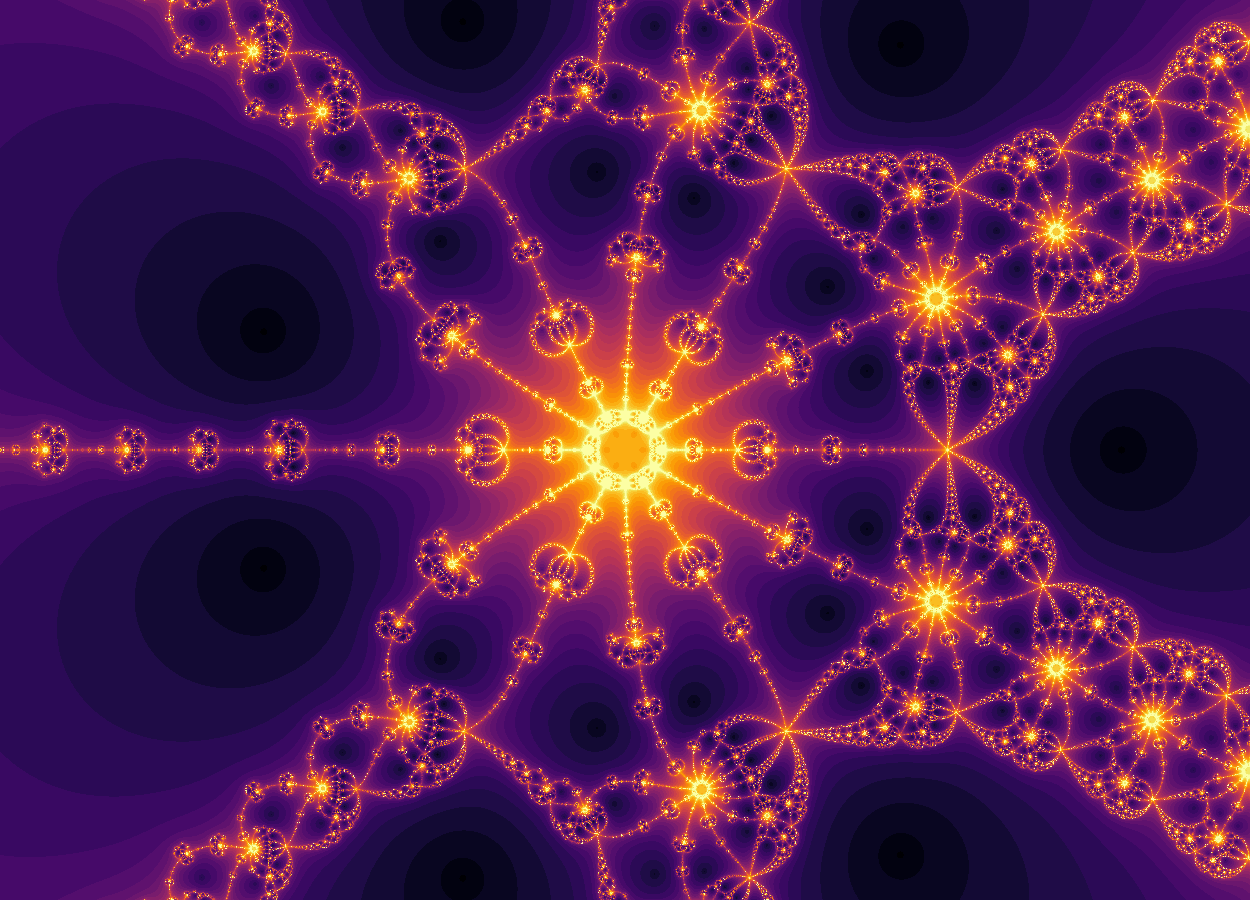
\includegraphics[scale=0.26]{images/ej1.png}
    \caption{Fractal generado por $x^7-x-1$}
    \label{fig:ej_1}
\end{figure}

\textbf{Función:}$x^6-x^3+11$

\textbf{Raíces:}

\begin{center}
\begin{tabular}{ c c }
 (-1.2523-0.8098i) & (-1.2523+0.8098i) \\
 (-0.0752-1.4894i) & (-0.0752+1.4894i) \\
 (1.3275-0.6796i) & (1.3275+0.6796i)
\end{tabular}
\end{center}

\begin{figure}[H]
    \centering
    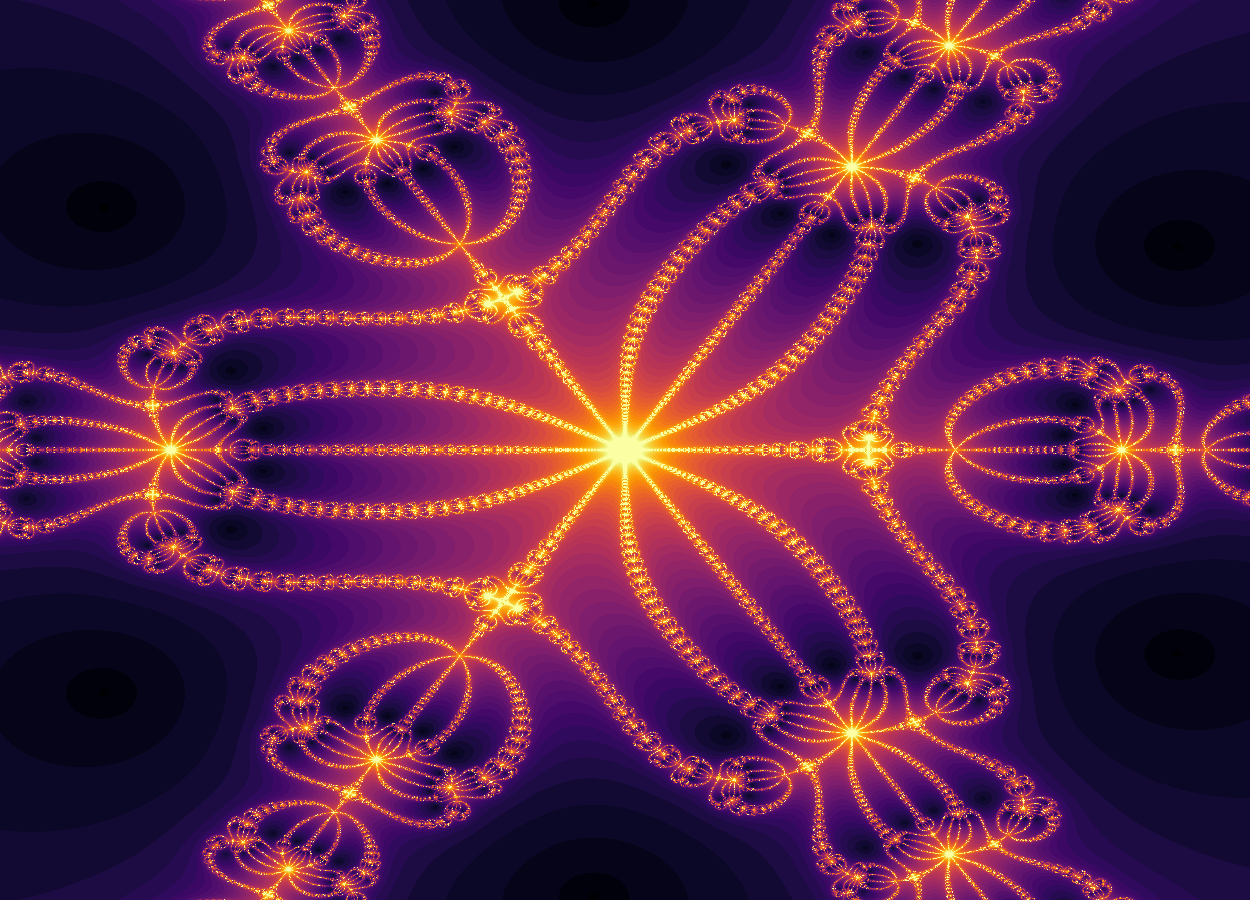
\includegraphics[scale=0.26]{images/ej2.png}
    \caption{Fractal generado por $x^6-x^3+11$}
    \label{fig:ej_2}
\end{figure}

\textbf{Función:}$x^4-x^2-1$

\textbf{Raíces:}

\begin{center}
\begin{tabular}{ c c  }
 (-1.272+0i) & (-0-0.7862i) \\
 0.7862i & (1.272+0i)
\end{tabular}
\end{center}

\begin{figure}[H]
    \centering
    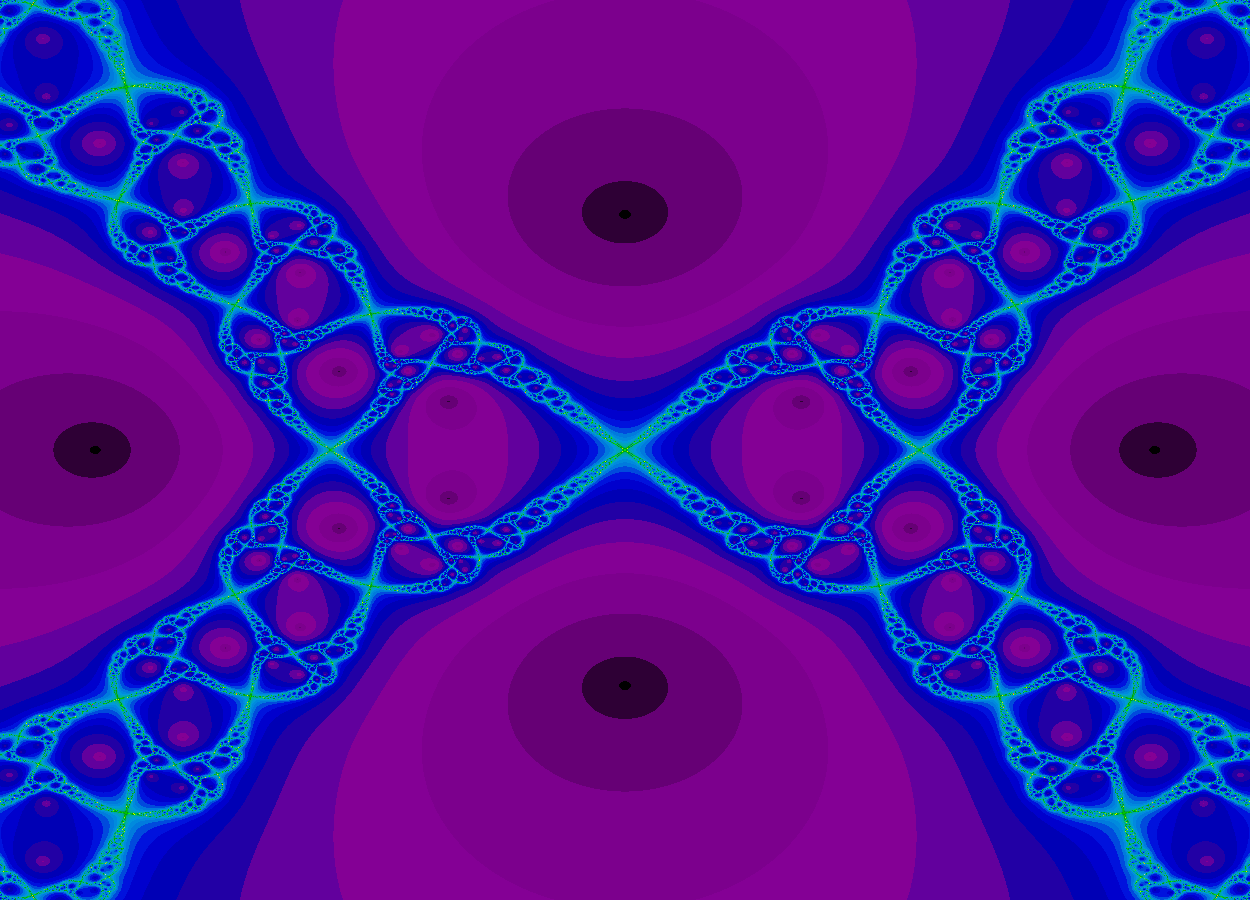
\includegraphics[scale=0.26]{images/ej3.png}
    \caption{Fractal generado por $x^4-x^2-1$}
    \label{fig:ej_3}
\end{figure}

\textbf{Función:}$x^6-3x^2-2x$

\textbf{Raíces:}

\begin{center}
\begin{tabular}{ c c  }
    (-1+0i) & (-0.7413+0i) \\ 
    0i & (0.1472-1.3576i) \\ 
    (0.1472+1.3576i) & (1.4469+0i)
 
\end{tabular}
\end{center}

\begin{figure}[H]
    \centering
    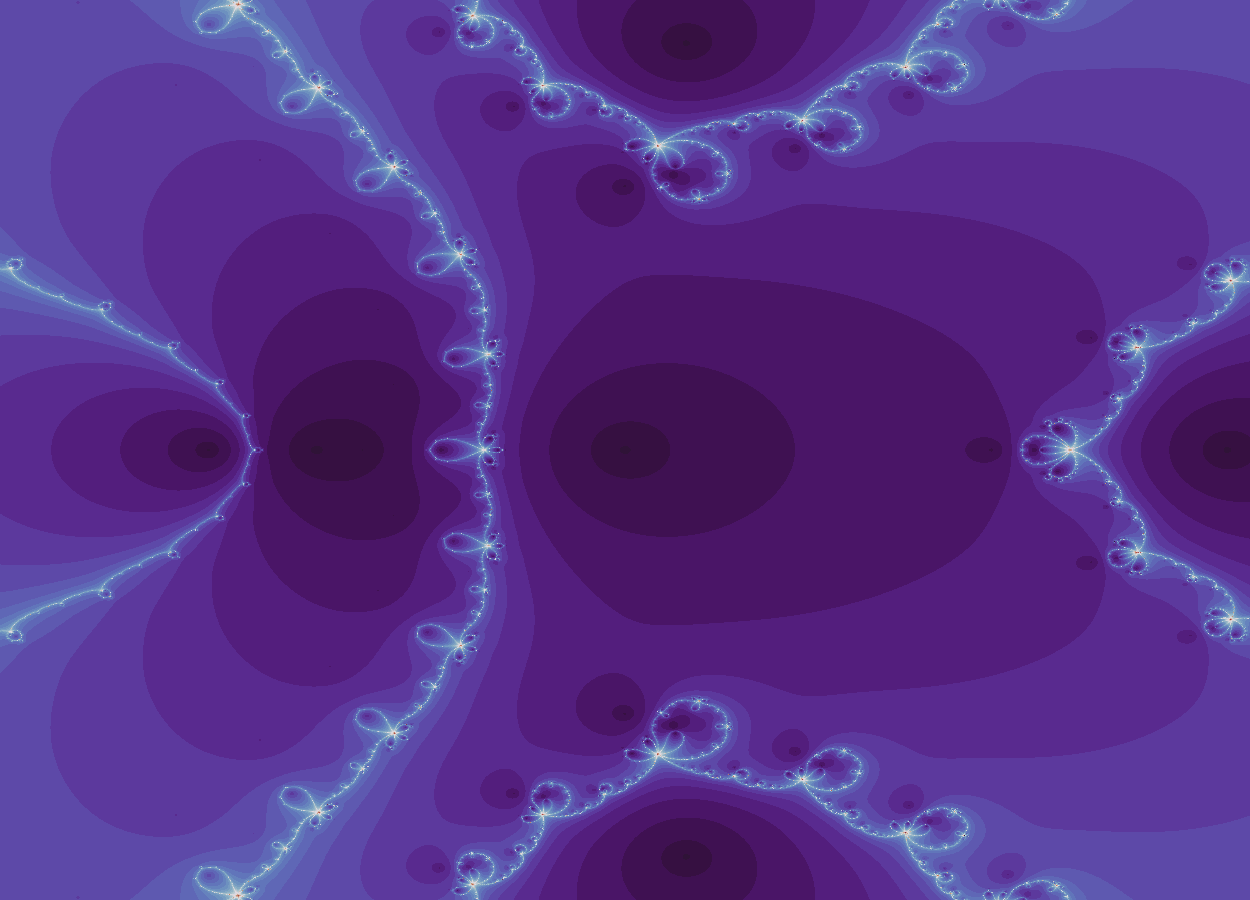
\includegraphics[scale=0.26]{images/ej4.png}
    \caption{Fractal generado por $x^6-3x^2-2x$}
    \label{fig:ej_4}
\end{figure}

\textbf{Función:}$x^7-x^2+1$

\textbf{Raíces:}

\begin{center}
\begin{tabular}{ c c  }
 (-0.8398+0i) & (-0.7555-0.7411i) \\ 
 (-0.7555+0.7411i) & (0.2945-1.0774i) \\ 
 (0.2945+1.0774i) & (0.8809-0.2758i) \\
 (0.8809+0.2758i)
\end{tabular}
\end{center}

\begin{figure}[H]
    \centering
    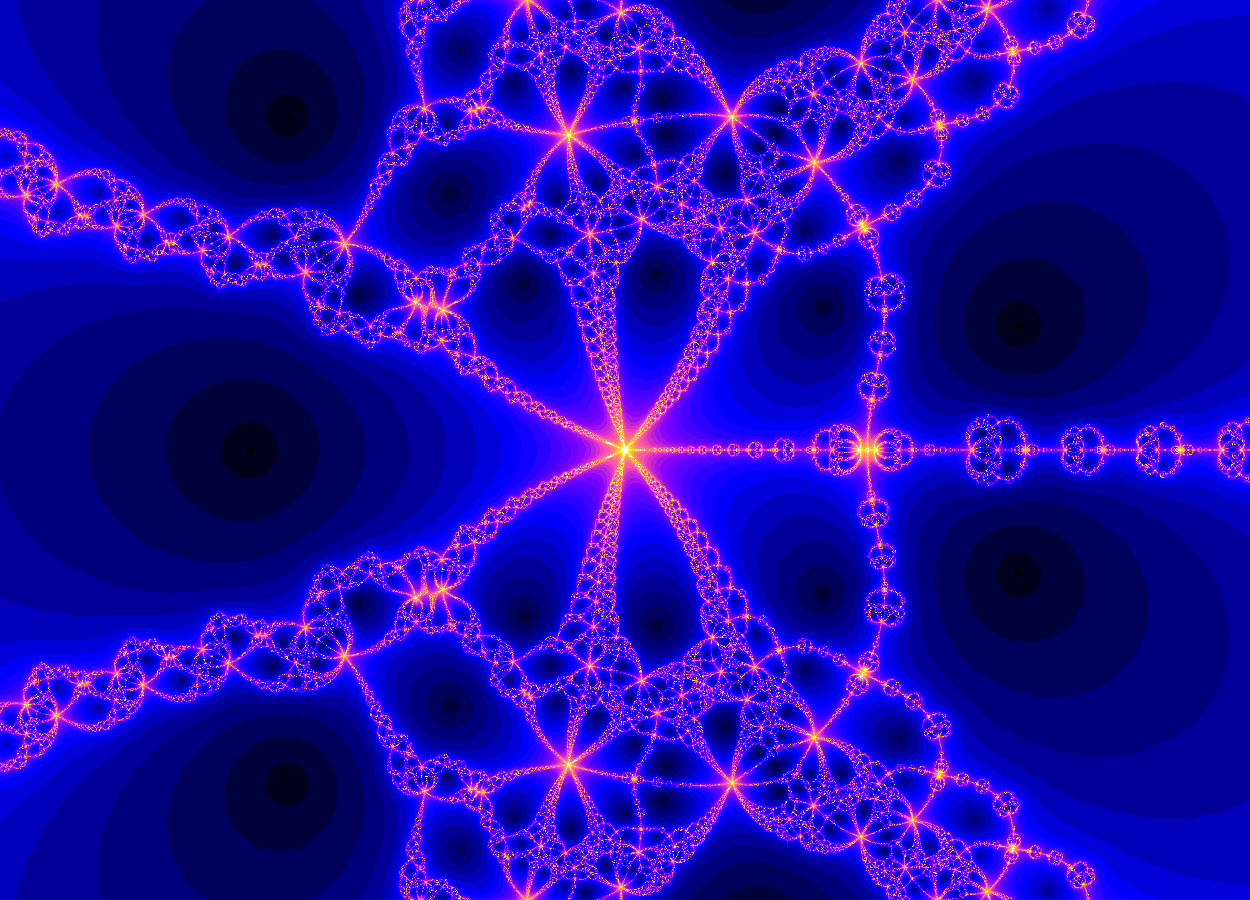
\includegraphics[scale=0.26]{images/ej5.png}
    \caption{Fractal generado por $x^7-x^2+1$}
    \label{fig:ej_5}
\end{figure}

\section{Referencias}


\bibliographystyle{plain}
\bibliography{ref}
\end{document}